\chapter{Physics Object and Event Selection}\label{sec:selection}
This chapter outlines the basic \hzg{} physics object and event selection before any event categorization is done.
Along the way, we will also point out the most relevant corrections applied, including trigger scale factors (SFs), physics object energy and momentum corrections, and identification and isolation SFs.

\section{Primary Vertex}
Events are required to have at least one good PV
with a reconstructed longitudinal position within 24\cm of the
geometric center of the detector and a transverse position within
2\cm of the nominal beam collision point. 
To avoid fake vertices, the PV reconstruction is required to have more than four degrees of freedom.
In the case of multiple satisfactory vertices, the vertex with the highest scalar sum of squared \pt is chosen.

\section{Triggers}
The topology and kinematics of the \hzg{} process guide the choice of triggers used in this analysis. As there are at least three final state decay products, 
the photon \pt tends to be less than in other channels, such as \hgg. Consequently, the CMS single photon trigger \pt thresholds 
are too great to make them viable options. In addition, there is no suitable unprescaled multijet plus photon trigger to target events with 
hadronic decays of the $\PZ$ boson, so the triggers are chosen to target the $\lplm\gamma$ final states.
Therefore, we trigger on the leptons arising from the decay of the Z boson, which tend 
to have larger values of \pt. The best approach to maximize signal efficiency is to use the double lepton triggers. 
The dielectron trigger requires a leading (subleading) electron with
$\pt > 23\,(12)\GeV$, while the dimuon trigger requires a muon with $\pt > 17\,(8)\GeV$. Events passing both the double muon and double electron triggers are classified as $\mpmm\gamma$ events.

The triggers are applied to both data and simulation. Trigger efficiencies and SFs are measured using the 
simulation samples corresponding to each data-taking year. These measurements use a tag and probe~\cite{cite:tagandprobe} method. 
This method takes advantage of the high purity of $\PZ\to\lplm$ events near the $\PZ$ boson mass peak. 
One lepton functions as the tag, and satisfies a set of tight trigger, identification, isolation, and \pt requirements. 
The second lepton, the probe, must pass a looser selection and is used to measure the efficiency in question. 
Using this approach, trigger efficiencies for each leg of a given double lepton trigger are measured in both data and simulation. 
Then a corrective SF, defined as the ratio of data efficiency to simulation efficiency, is applied to the simulation. 
Scale factors are measured and applied in bins of \pt and $|\eta|$.

For the double electron trigger efficiency measurements, the tag electron must satisfy a set of requirements. The tag must pass 
the single electron trigger, pass a tight cut-based identification, have $\pt>30\,(35)\GeV$ in 2016 (2017 and 2018), and have $|\eta|<2.5$. 
The probe electron must pass a loose electron MVA identification requirement. The details of the electron MVA identification will be described later in this chapter.
The efficiencies for each leg 
of the trigger are measured separately, so in each case, the probe electron must match the trigger leg being measured. 
The efficiencies for each double electron trigger leg for 2016, 2017, and 2018 are shown in Fig. \ref{fig:ele_trig_SF}.
On average, the double electron trigger efficiency is measured to be in the range of 86--97\%, depending on the electron \pt and $\eta$.

\begin{figure}[tb]
	\begin{center}
		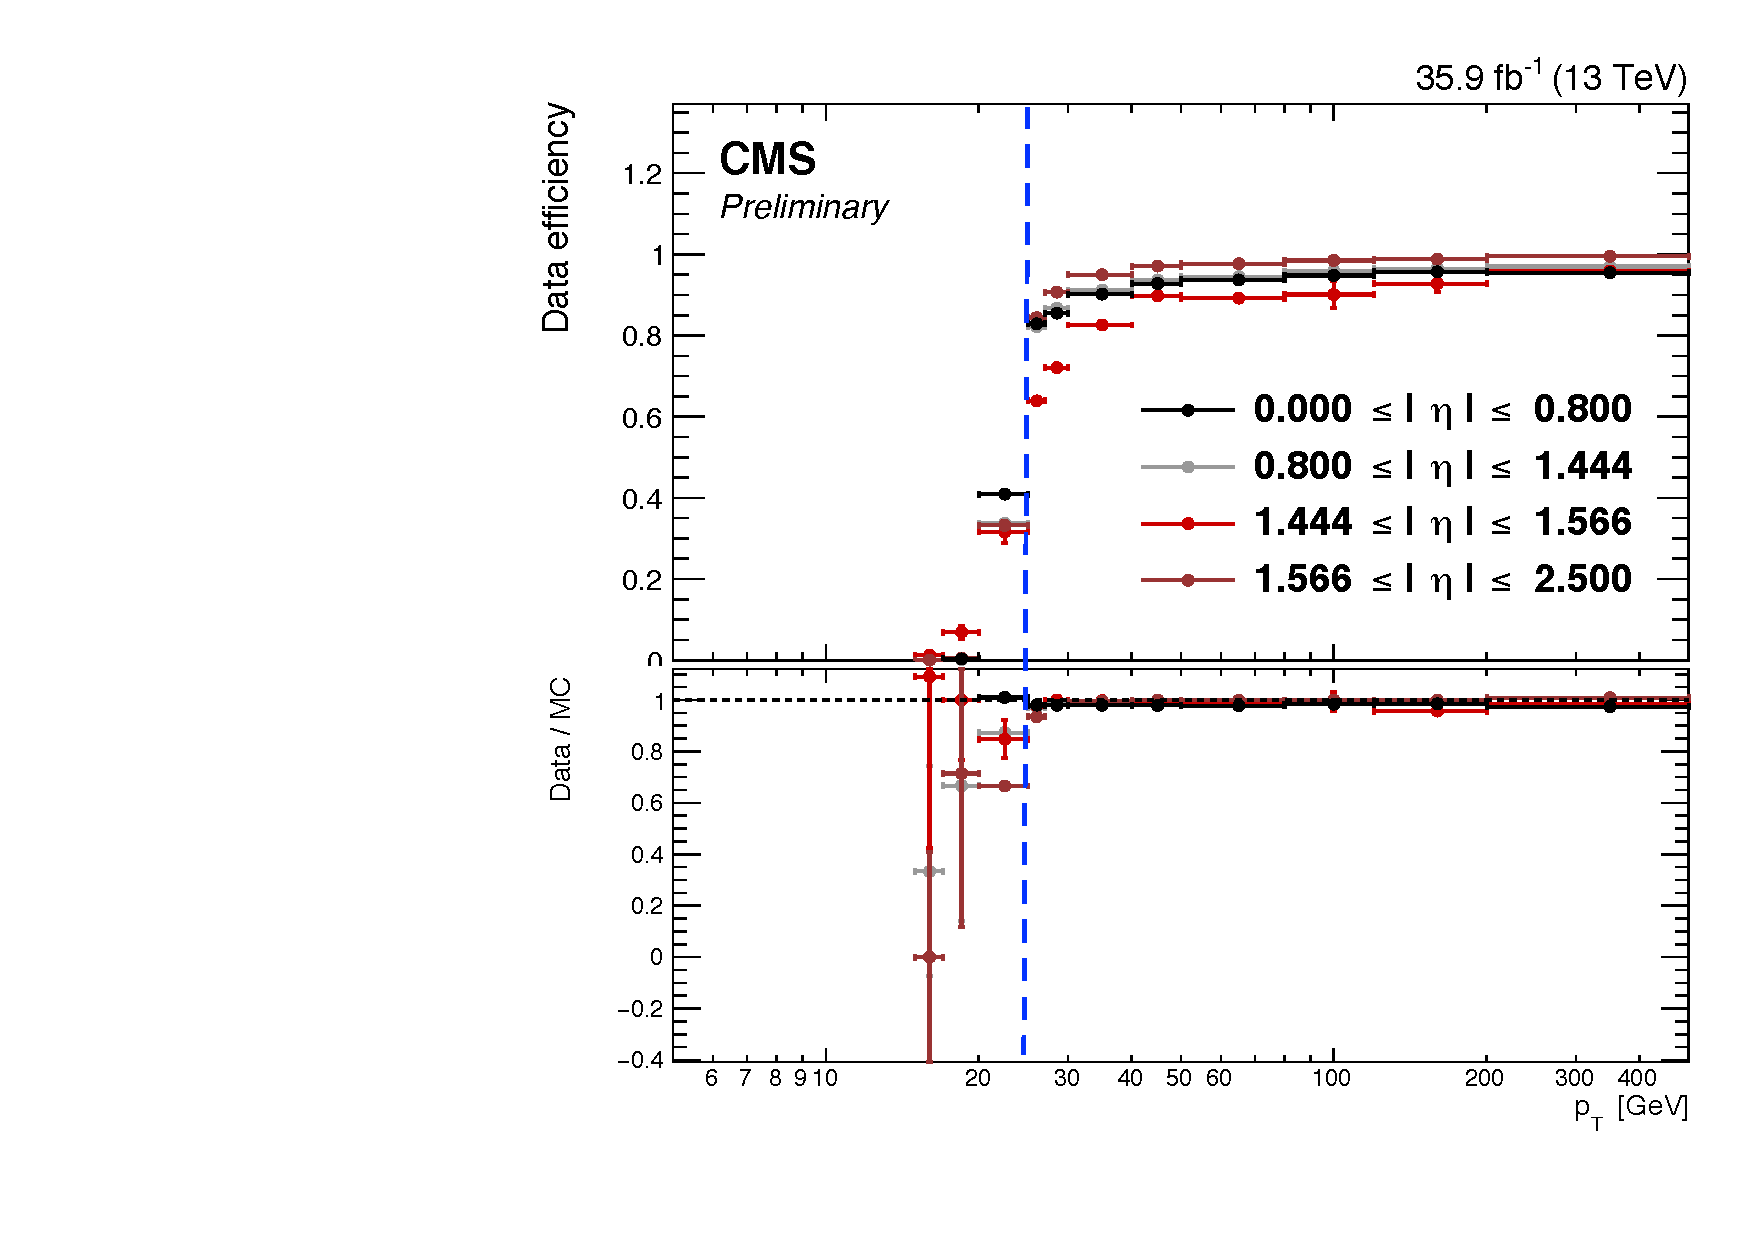
\includegraphics[width=0.30\textwidth]{fig/SFs/2016_ele_trg1_1D.pdf}
		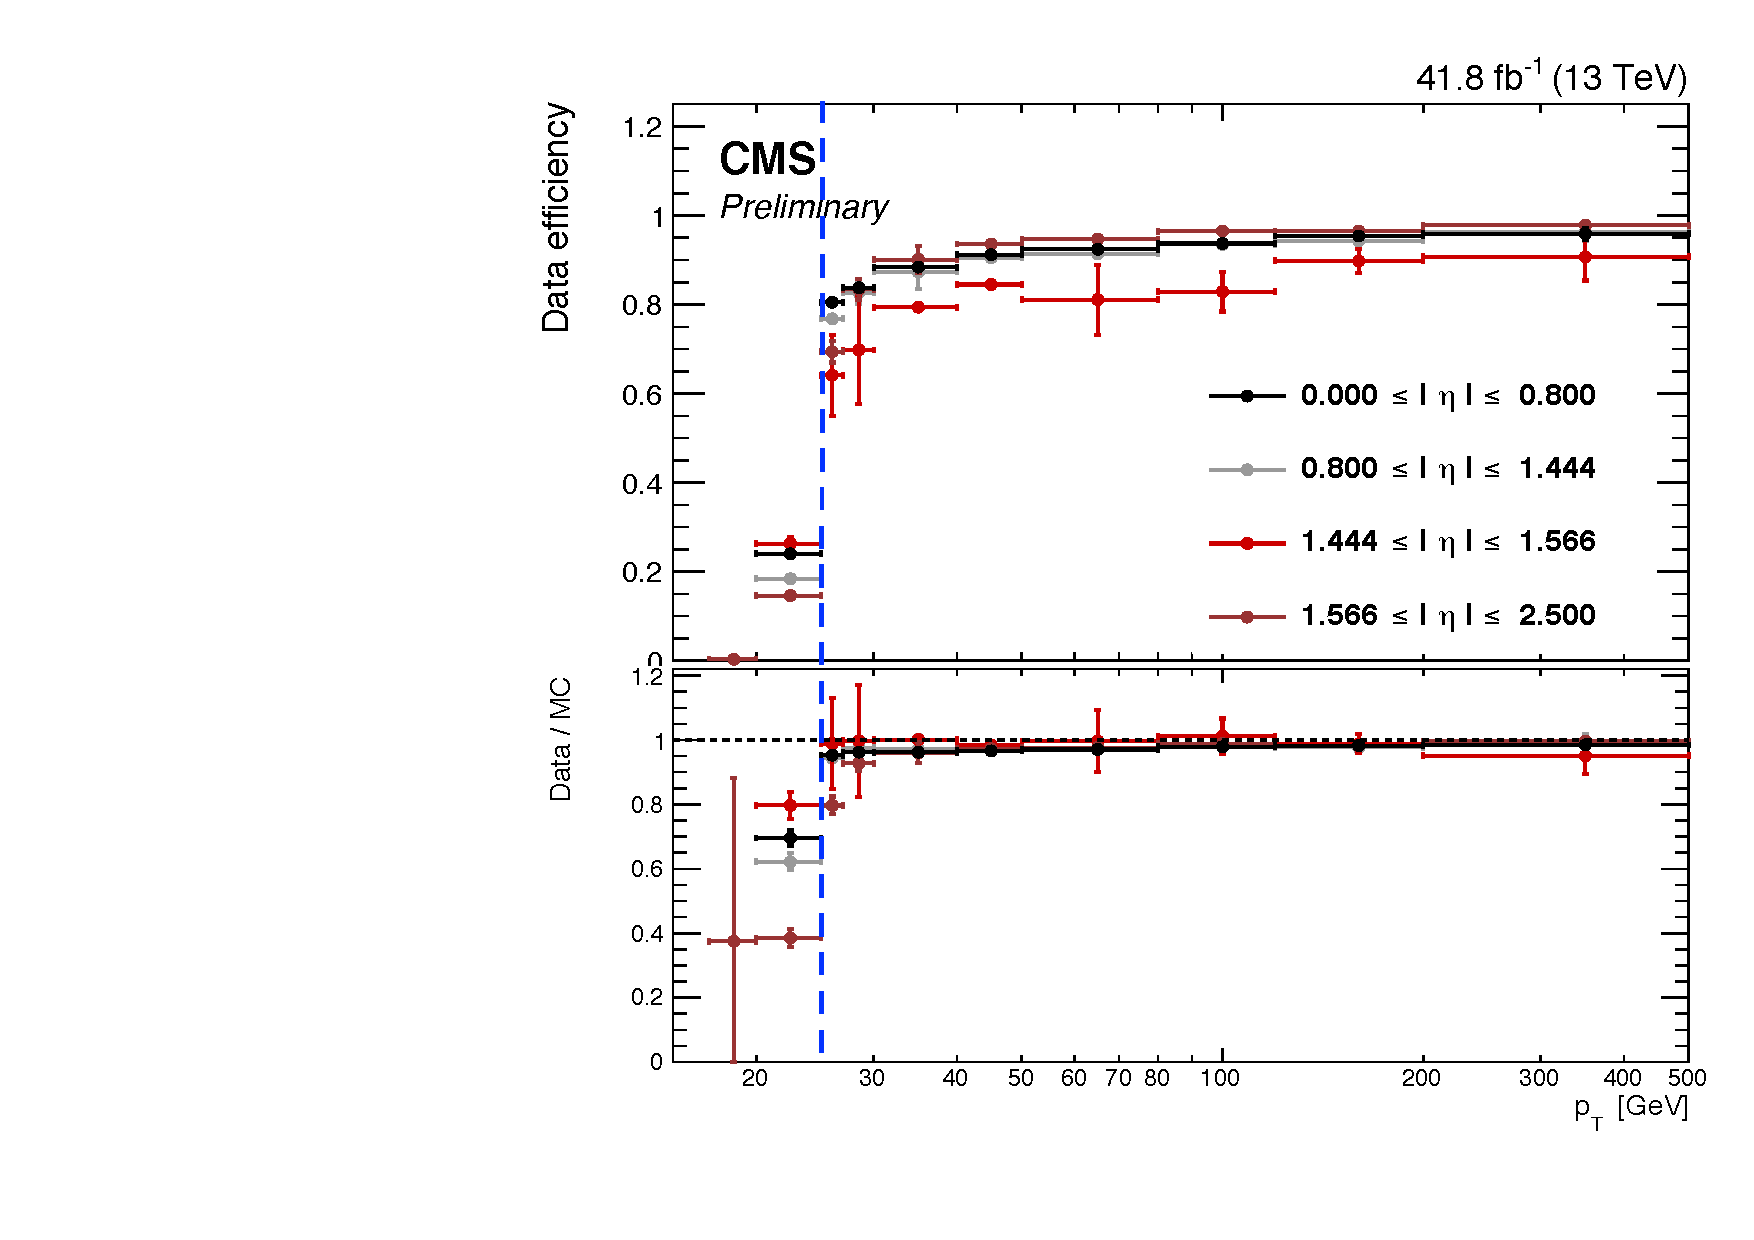
\includegraphics[width=0.30\textwidth]{fig/SFs/2017_ele_trg1_1D.pdf}
		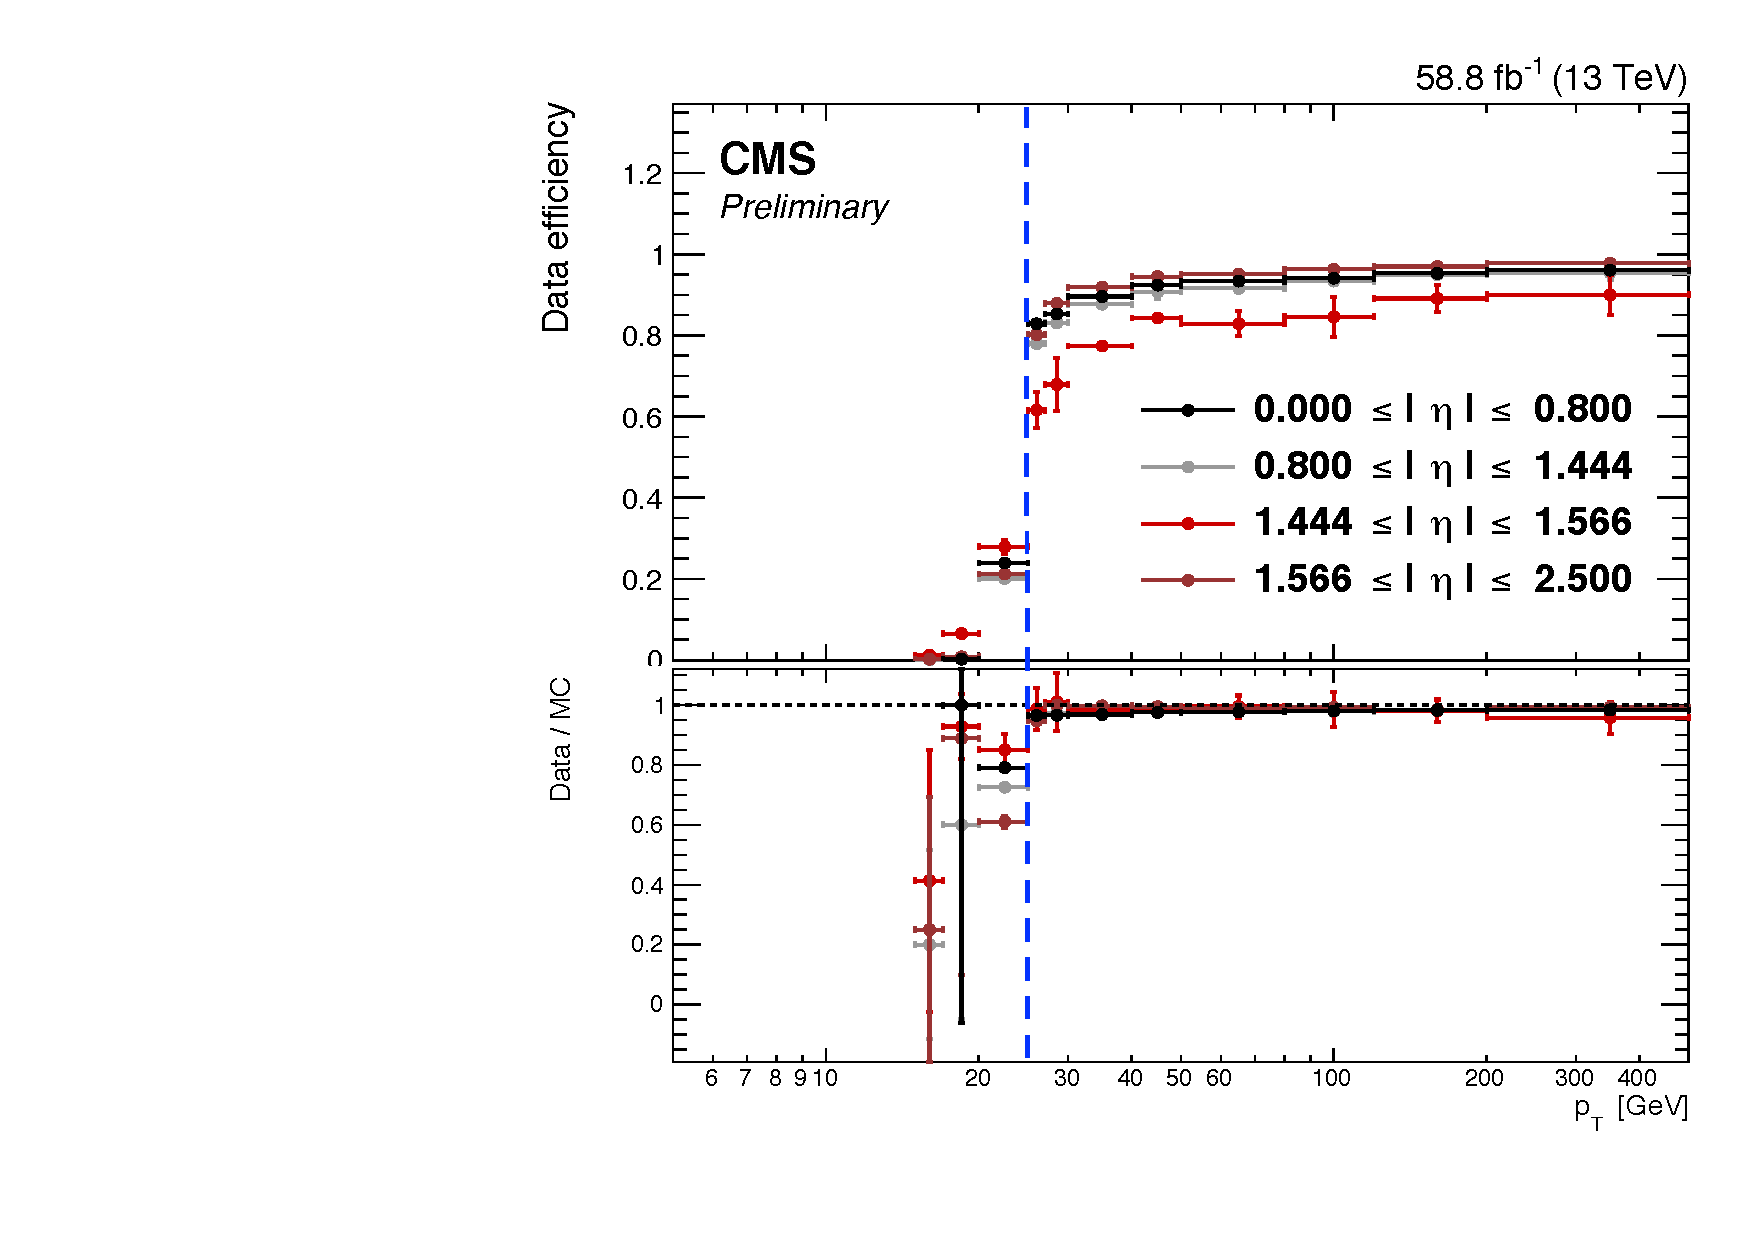
\includegraphics[width=0.30\textwidth]{fig/SFs/2018_ele_trg1_1D.pdf}
		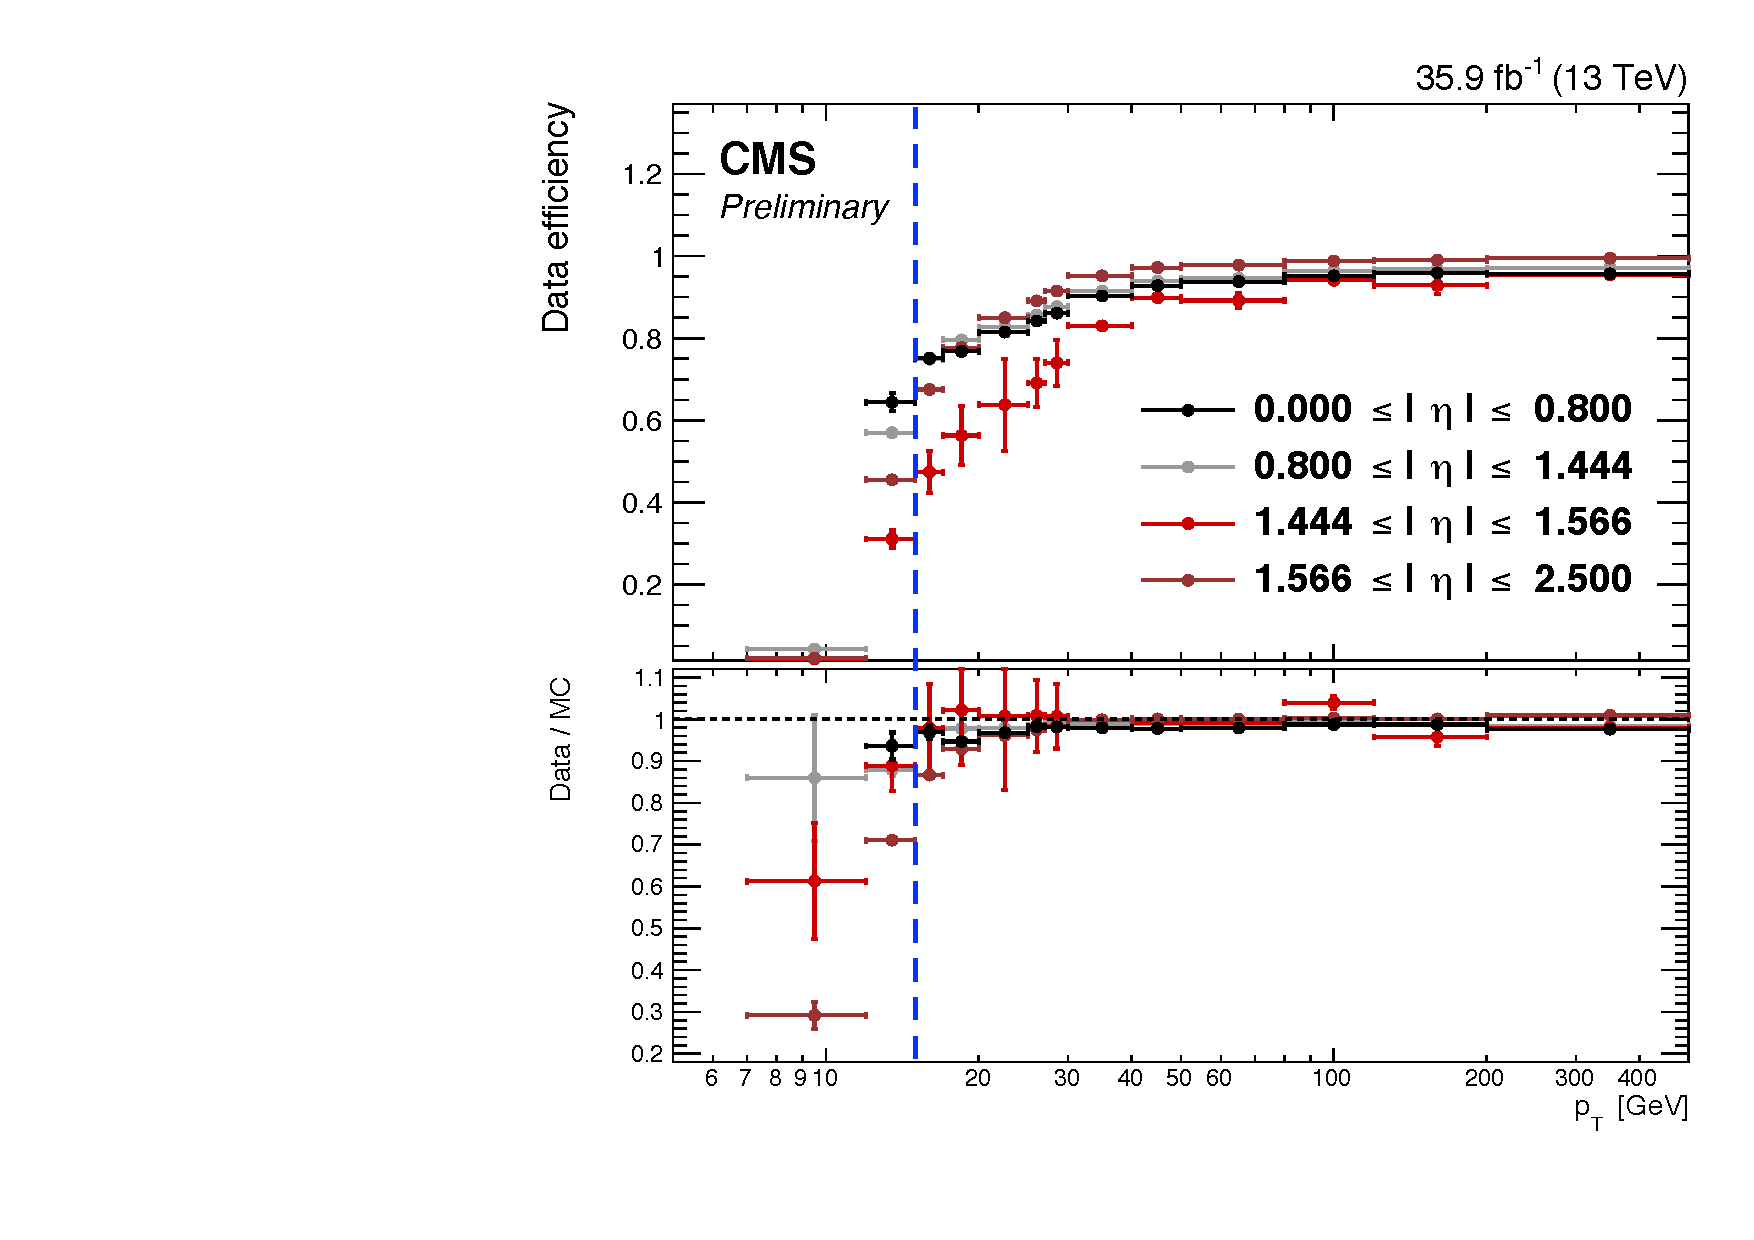
\includegraphics[width=0.30\textwidth]{fig/SFs/2016_ele_trg2_1D.pdf}
		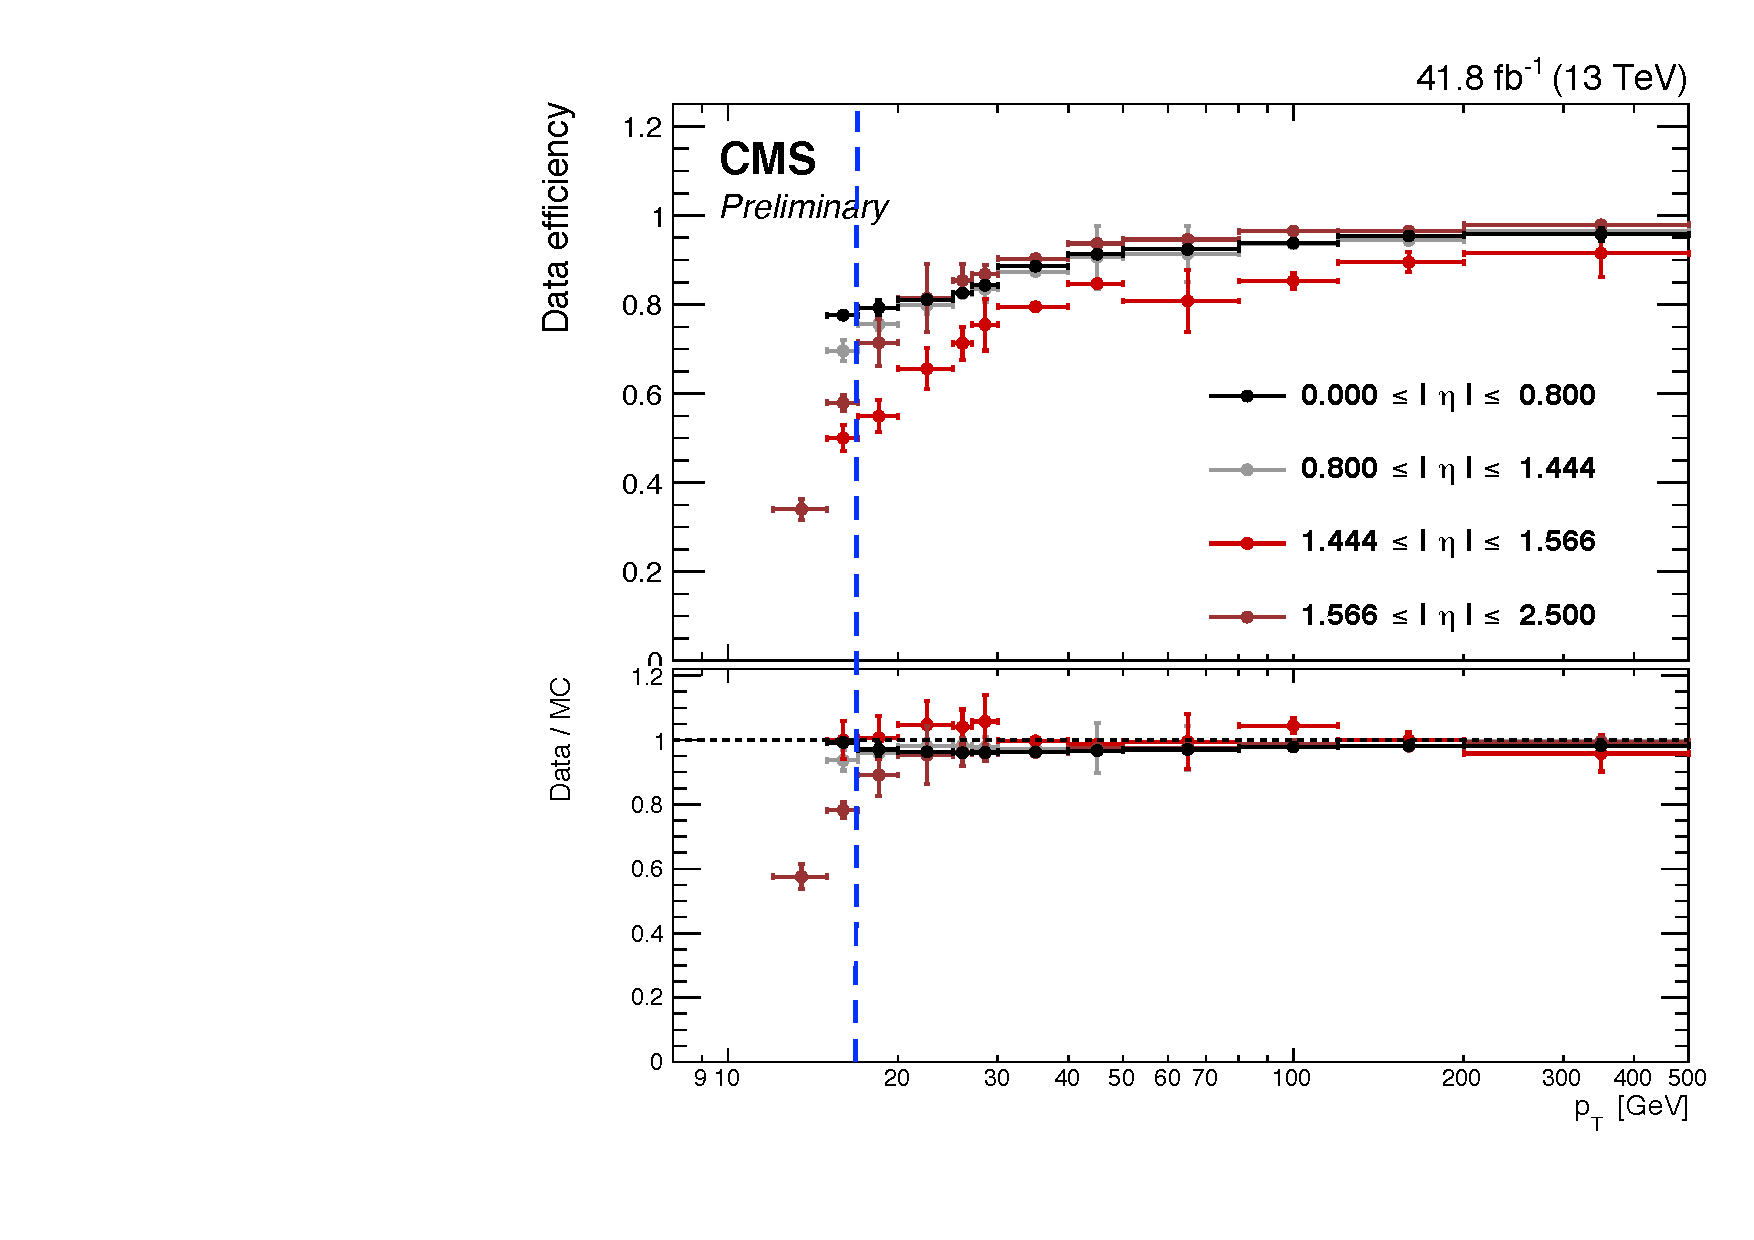
\includegraphics[width=0.30\textwidth]{fig/SFs/2017_ele_trg2_1D.pdf}
		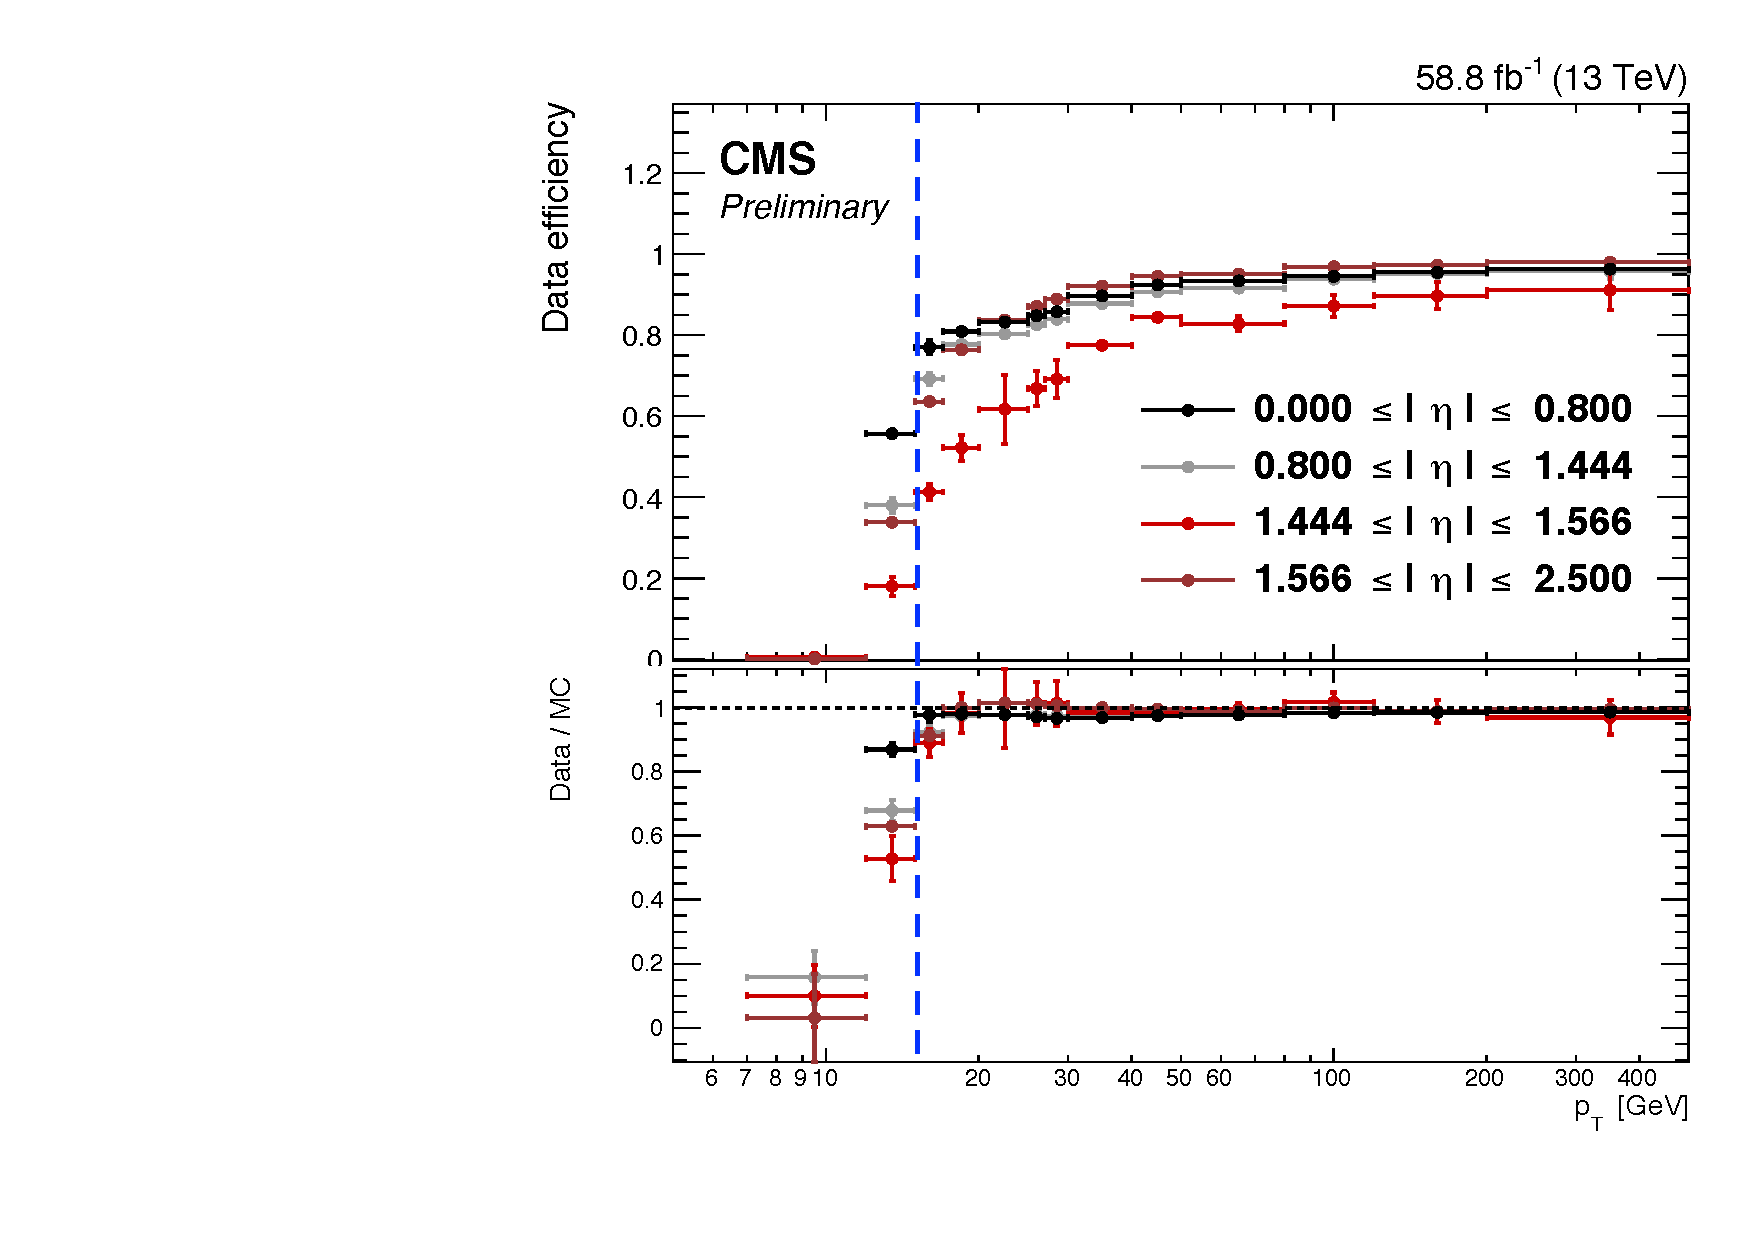
\includegraphics[width=0.30\textwidth]{fig/SFs/2018_ele_trg2_1D.pdf}
	\end{center}
	\caption{Efficiency measurements for each leg of the double electron trigger in 2016 (left), 2017 (center), and 2018 (right). The upper (lower) plots correspond to the 
	leading (subleading) trigger leg.}
	\label{fig:ele_trig_SF}
\end{figure}

For the double muon trigger efficiency measurements, the tag muon must satisfy a set of requirements. It must pass the single 
muon trigger, pass a tight cut-based identification, have $\pt>26\,(29)$ GeV for 2016 (2017 and 2018) and satisfy $|\eta| < 2.4$. The 
probe muon must pass the $\PH\to\PZ\PZ$ identification and isolation cuts. The details of the $\PH\to\PZ\PZ$ muon 
identification will be described later in this chapter. The efficiencies for each leg of the trigger are measured separately, so in each case, the probe 
muon must match the trigger leg being measured. The efficiencies for each double muon trigger leg for 2016, 2017, 
and 2018 are shown in Fig. \ref{fig:mu_trig_SF}. On average, the double muon trigger efficiency is measured to be in the range of 93--95\%, depending on the muon \pt and $\eta$.

\begin{figure}[tb]
	\begin{center}
		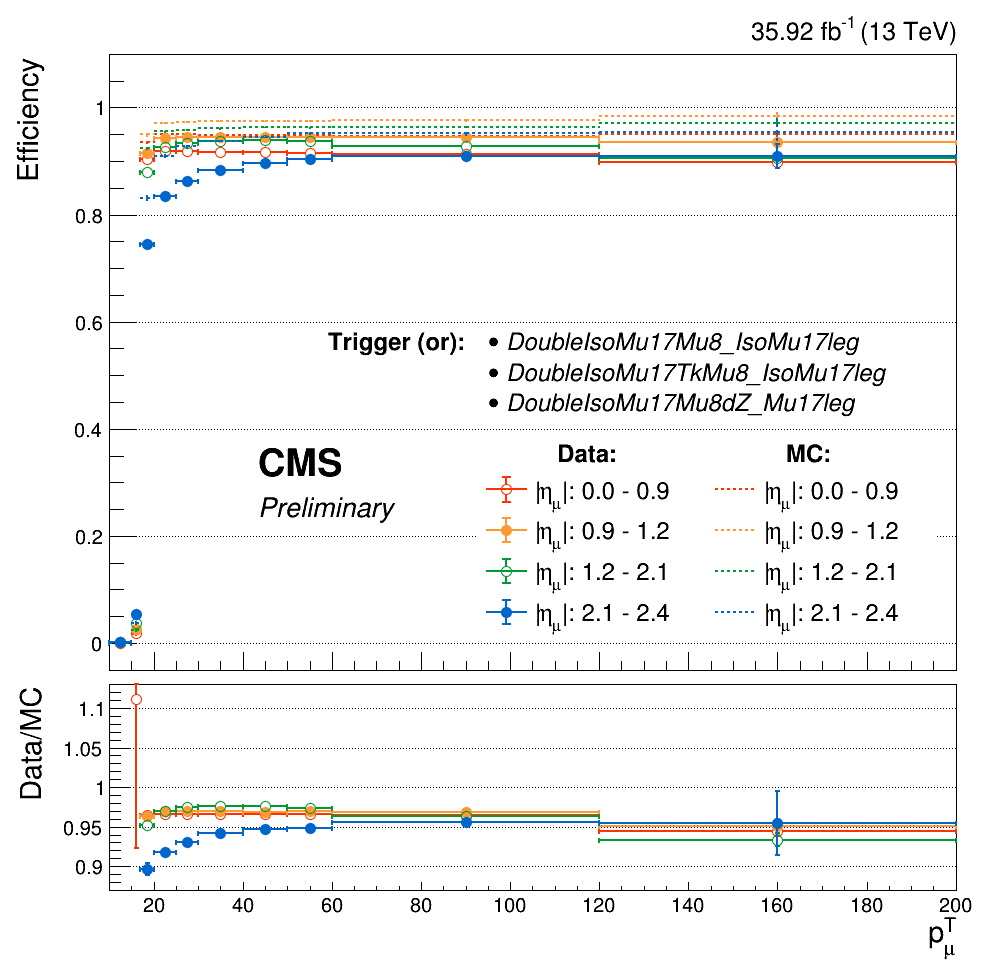
\includegraphics[width=0.30\textwidth]{fig/SFs/sf1D_year2016_leg1.png}
		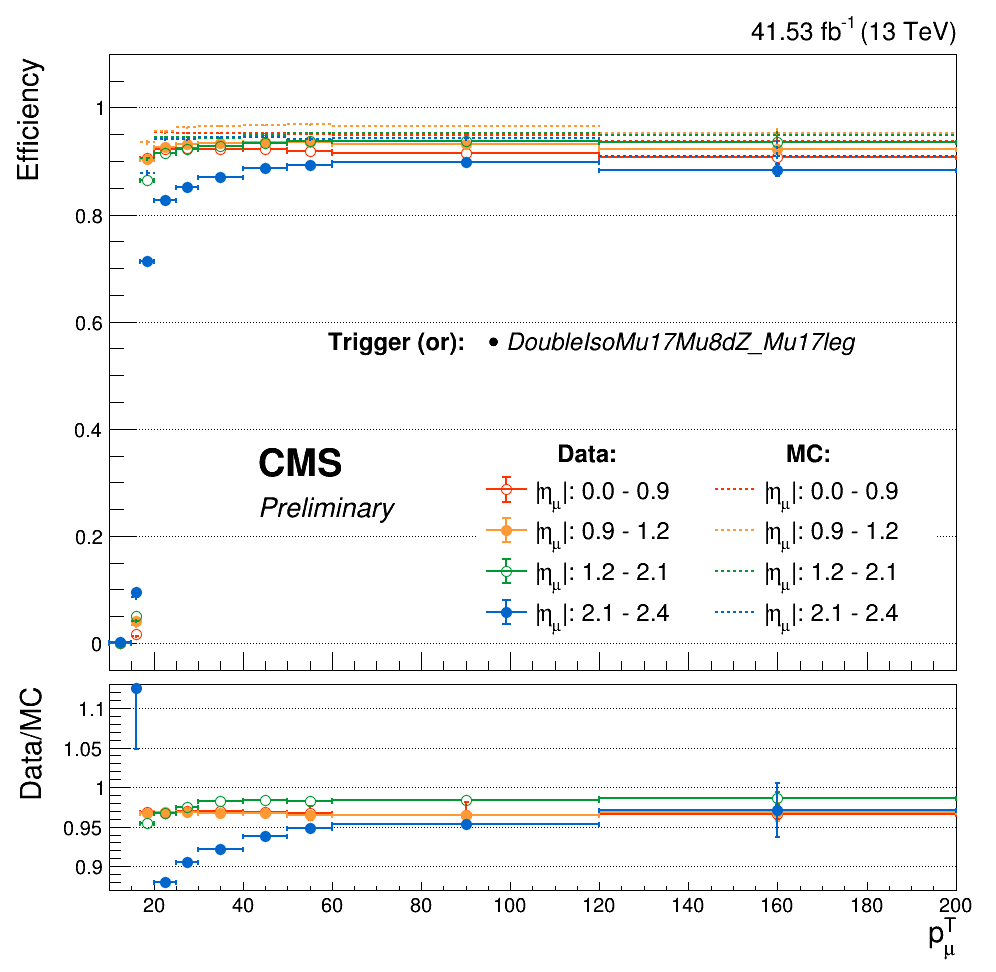
\includegraphics[width=0.30\textwidth]{fig/SFs/sf1D_year2017_leg1.png}
		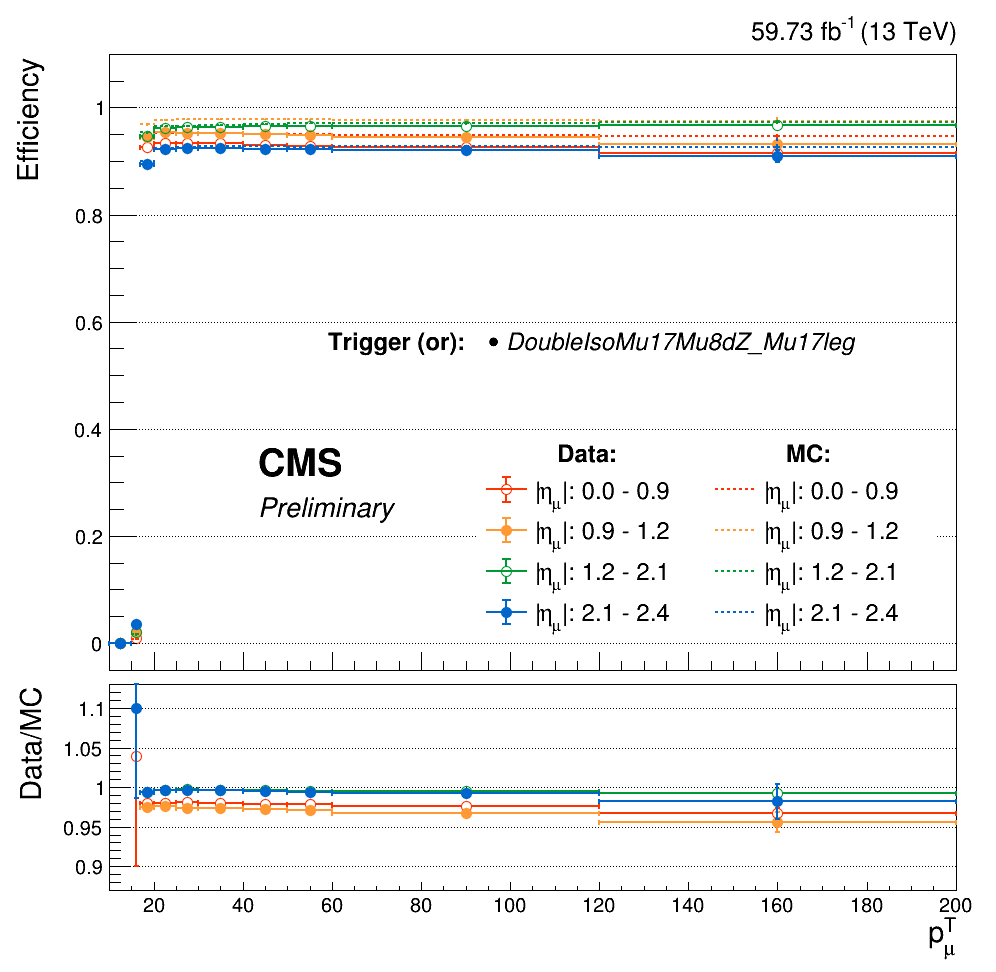
\includegraphics[width=0.30\textwidth]{fig/SFs/sf1D_year2018_leg1.png}
		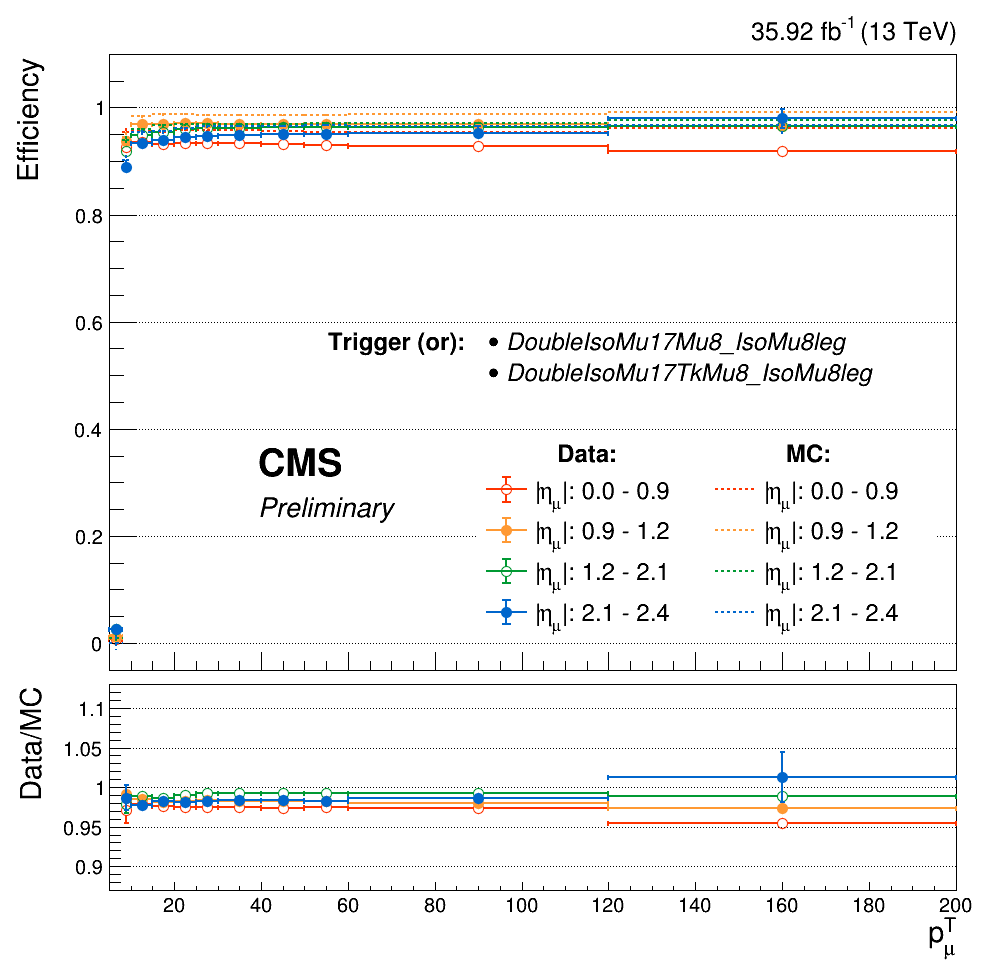
\includegraphics[width=0.30\textwidth]{fig/SFs/sf1D_year2016_leg2.png}
		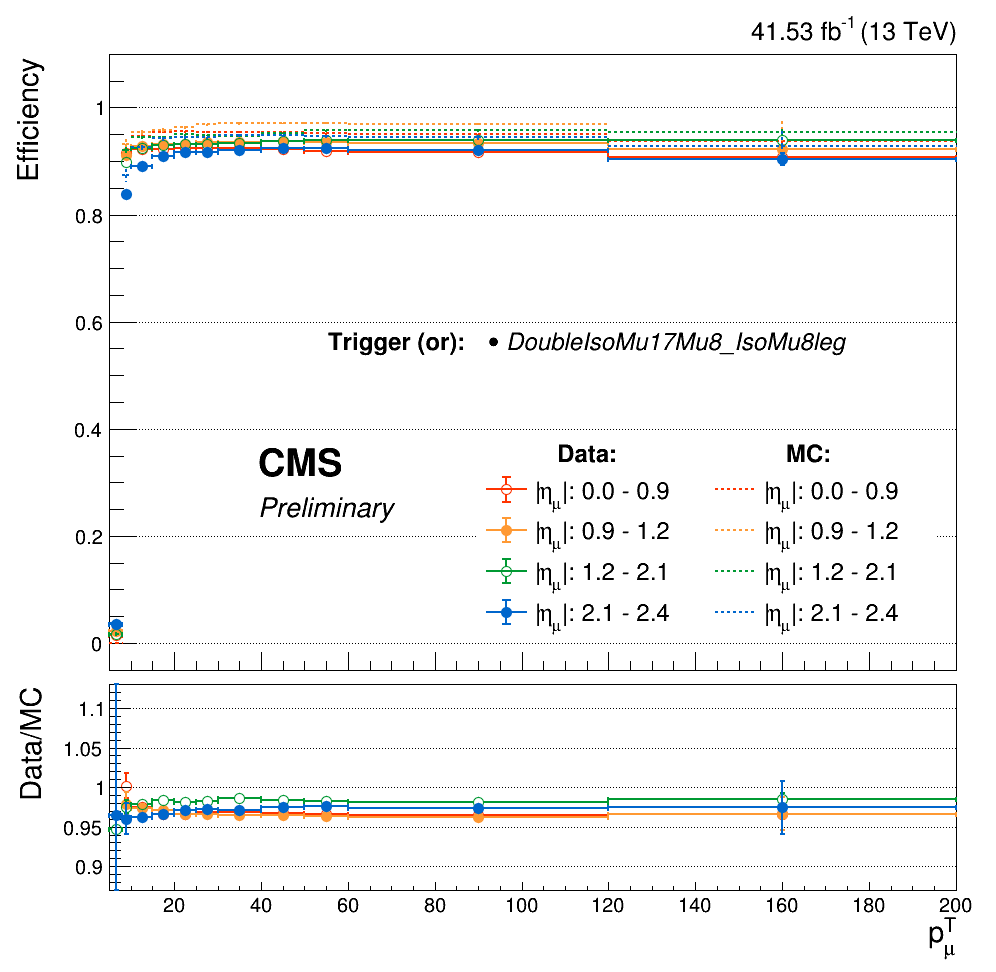
\includegraphics[width=0.30\textwidth]{fig/SFs/sf1D_year2017_leg2.png}
		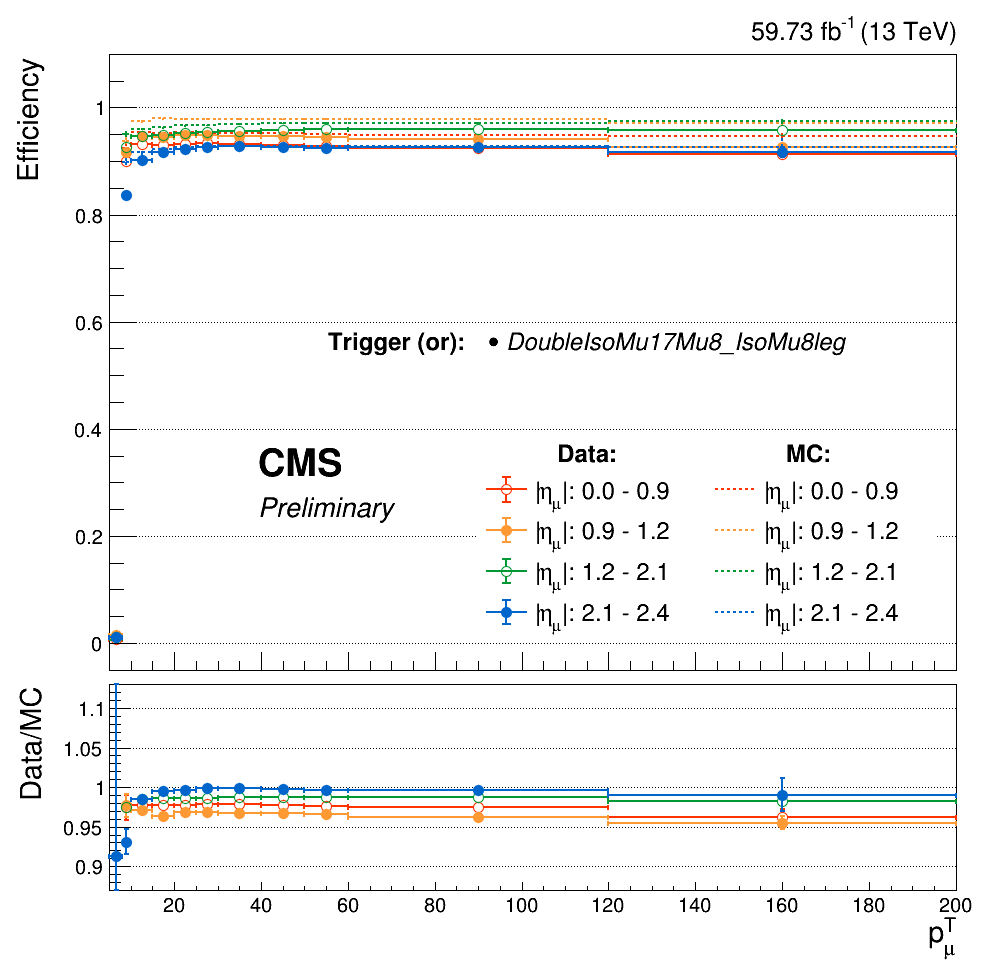
\includegraphics[width=0.30\textwidth]{fig/SFs/sf1D_year2018_leg2.png}
	\end{center}
	\caption{Efficiency measurements for each leg of the double muon trigger in 2016 (left), 2017 (center), and 2018 (right). The upper (lower) plots correspond to the 
	leading (subleading) trigger leg.}
	\label{fig:mu_trig_SF}
\end{figure}

\section{Photon Selection}
Photons are identified using a BDT discriminant (photon MVA ID) trained on $\PGg$+jets simulation in order to distinguish real photons from jets misreconstructed as photons. 
The features used for the BDT training include supercluster kinematics, isolation variables, and shower shape variables~\cite{EGM:PhotonID}. 
To reject electrons faking photons, a conversion-safe electron veto is also applied. In order to improve agreement between simulation and data for the photon MVA ID, shower 
shape corrections are taken from the CMS $\PH\to\PGg\PGg$ analysis of the same data set~\cite{CMS:2021kom} and applied to simulated events. 
The photon MVA ID is then reevaluated after these corrections. We correct the following features: $R_{9}^{5x5}$, defined as the ratio of energy in
the 5x5 array of ECAL crystals to the supercluster energy; $S_{4}$, defined as the ratio of the maximum energy 2x2 array to the energy of 
the 5x5 array; the energy weighted shower widths $\sigma_{\eta}$ and $\sigma_{\phi}$; the energy weighted widths by crystal index 
$\sigma_{i\eta i\eta}$ and $\sigma_{i\eta i\phi}$; photon isolation, charged isolation with respect to the primary vertex, 
and charged isolation with respect to the worst vertex choice. The validity of the shower shape corrections is checked using tag 
and probe procedures for $\PZ\to\epem$ events where the probe electron mimics a photon and $\PZ\to\mpmm$
events with an FSR photon. Comparisons of the agreement between uncorrected and corrected simulation with data for the photon MVA ID are shown in 
Fig. \ref{fig:photon_mva_correction}. Similar plots for individual shower shape features can be found in Appendix \ref{sec:shower_shape}. 

\begin{figure}[tb]
	\begin{center}
		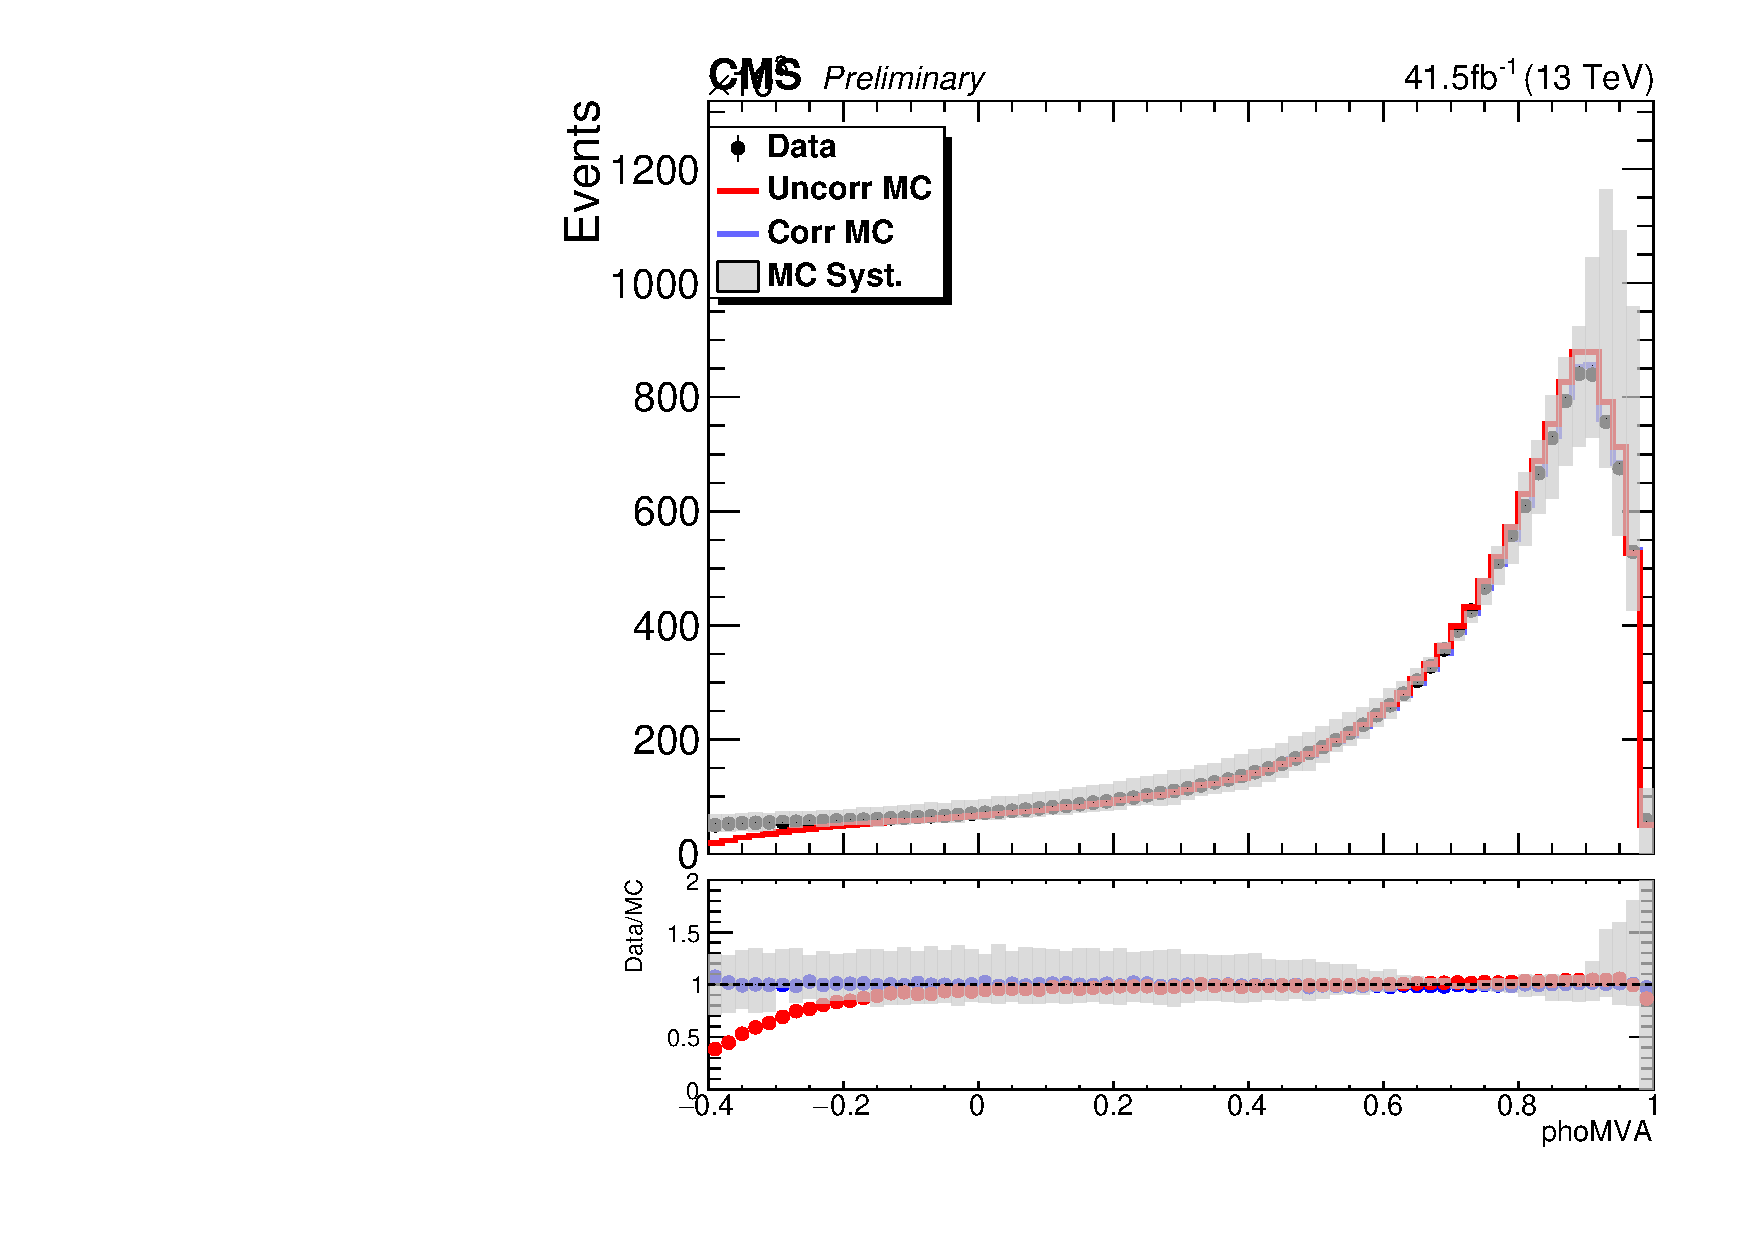
\includegraphics[width=0.35\textwidth]{fig/ss_corr/phoMVA_17_EB_Z.pdf}
		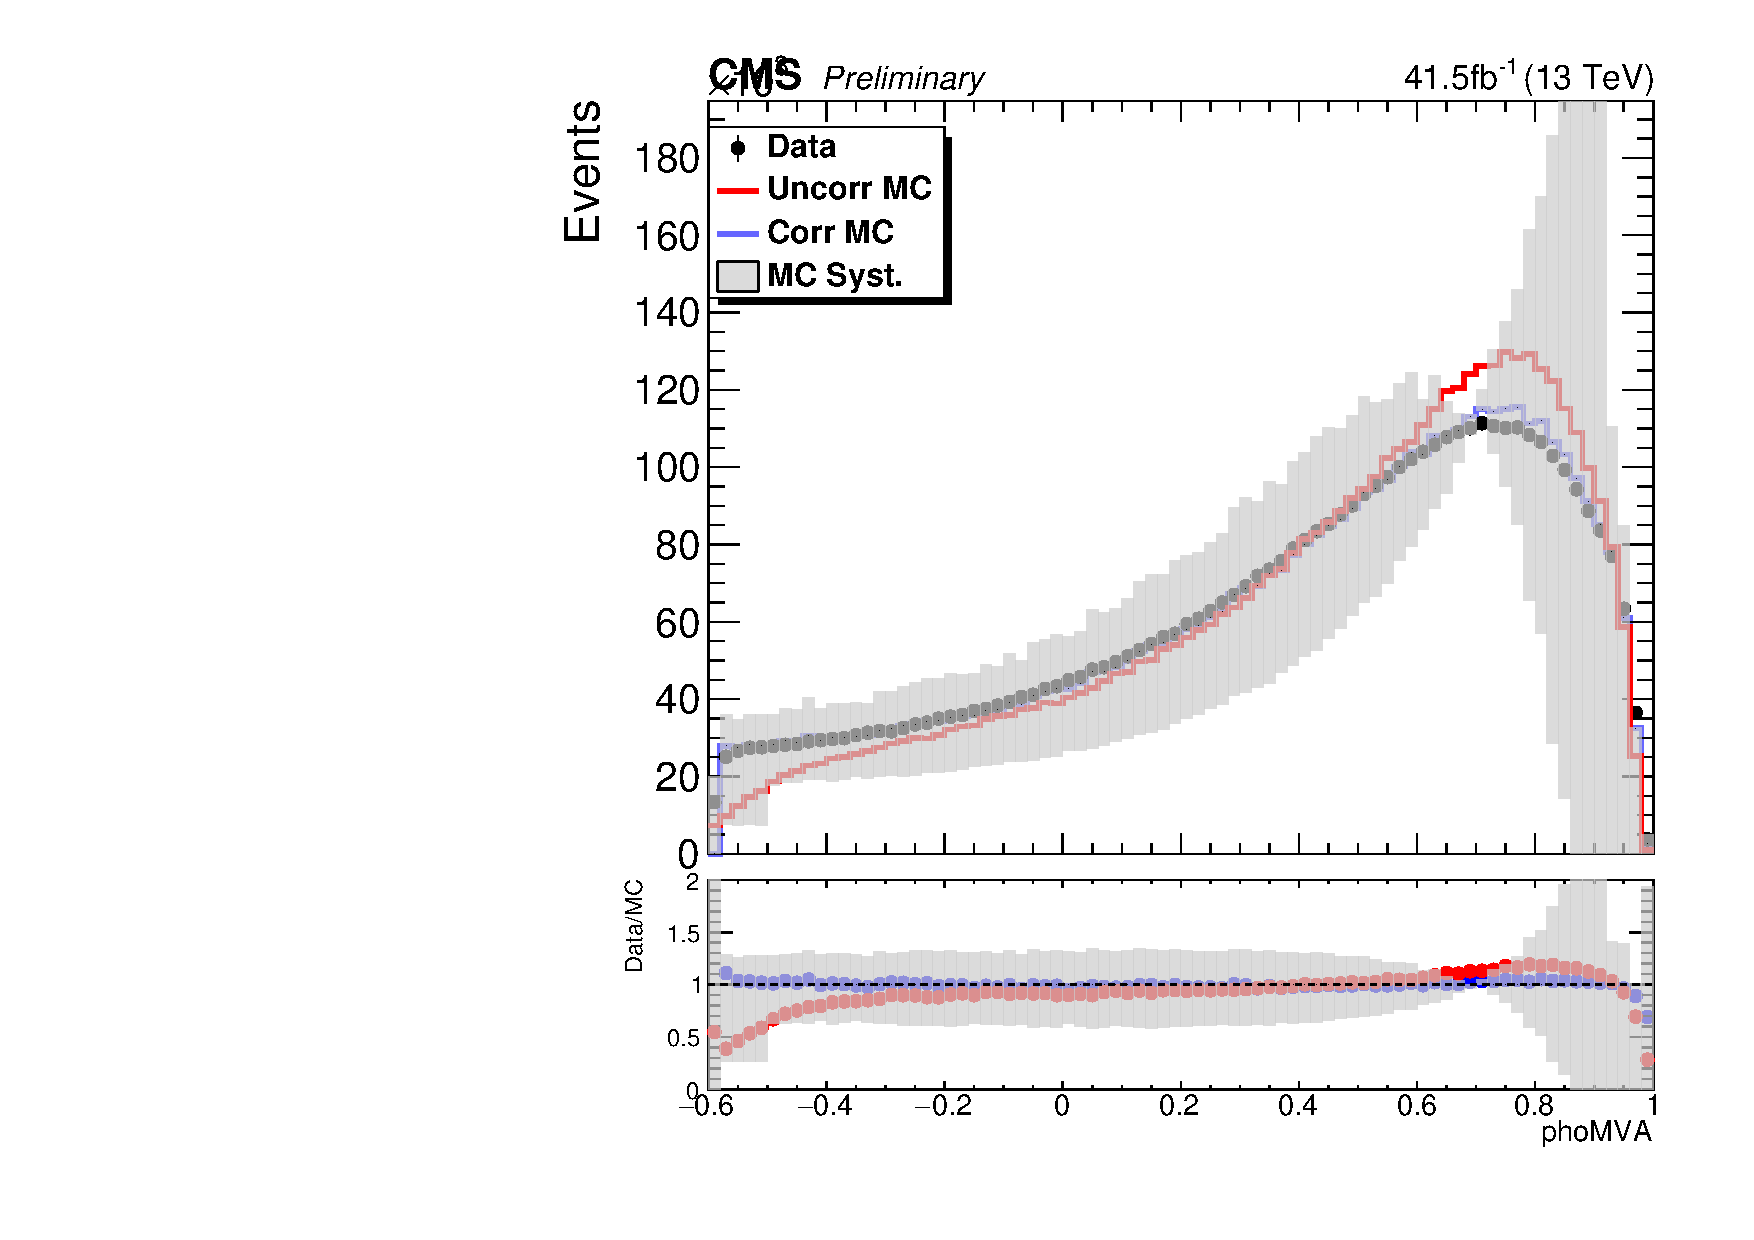
\includegraphics[width=0.35\textwidth]{fig/ss_corr/phoMVA_17_EE_Z.pdf}
		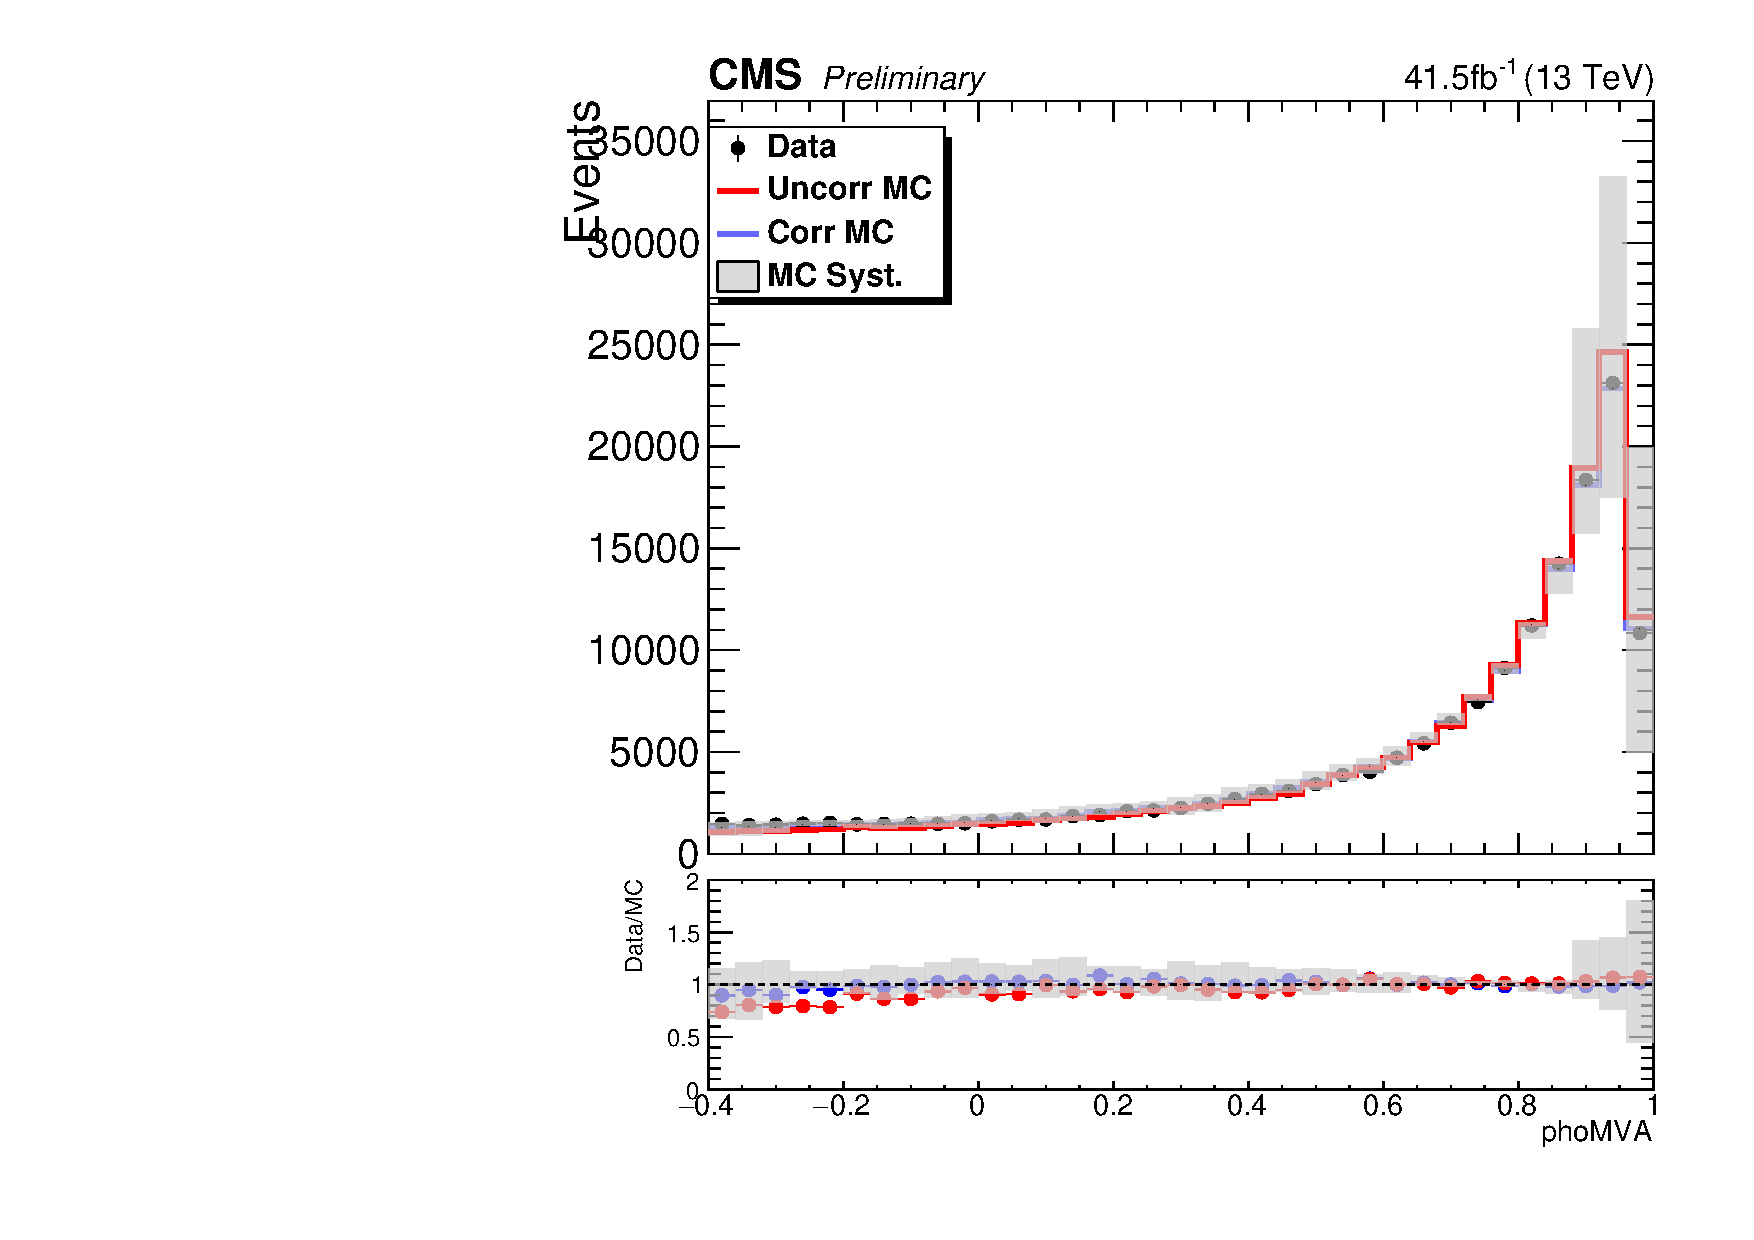
\includegraphics[width=0.35\textwidth]{fig/ss_corr/phoMVA_17_EB_Z_mmg.pdf}
		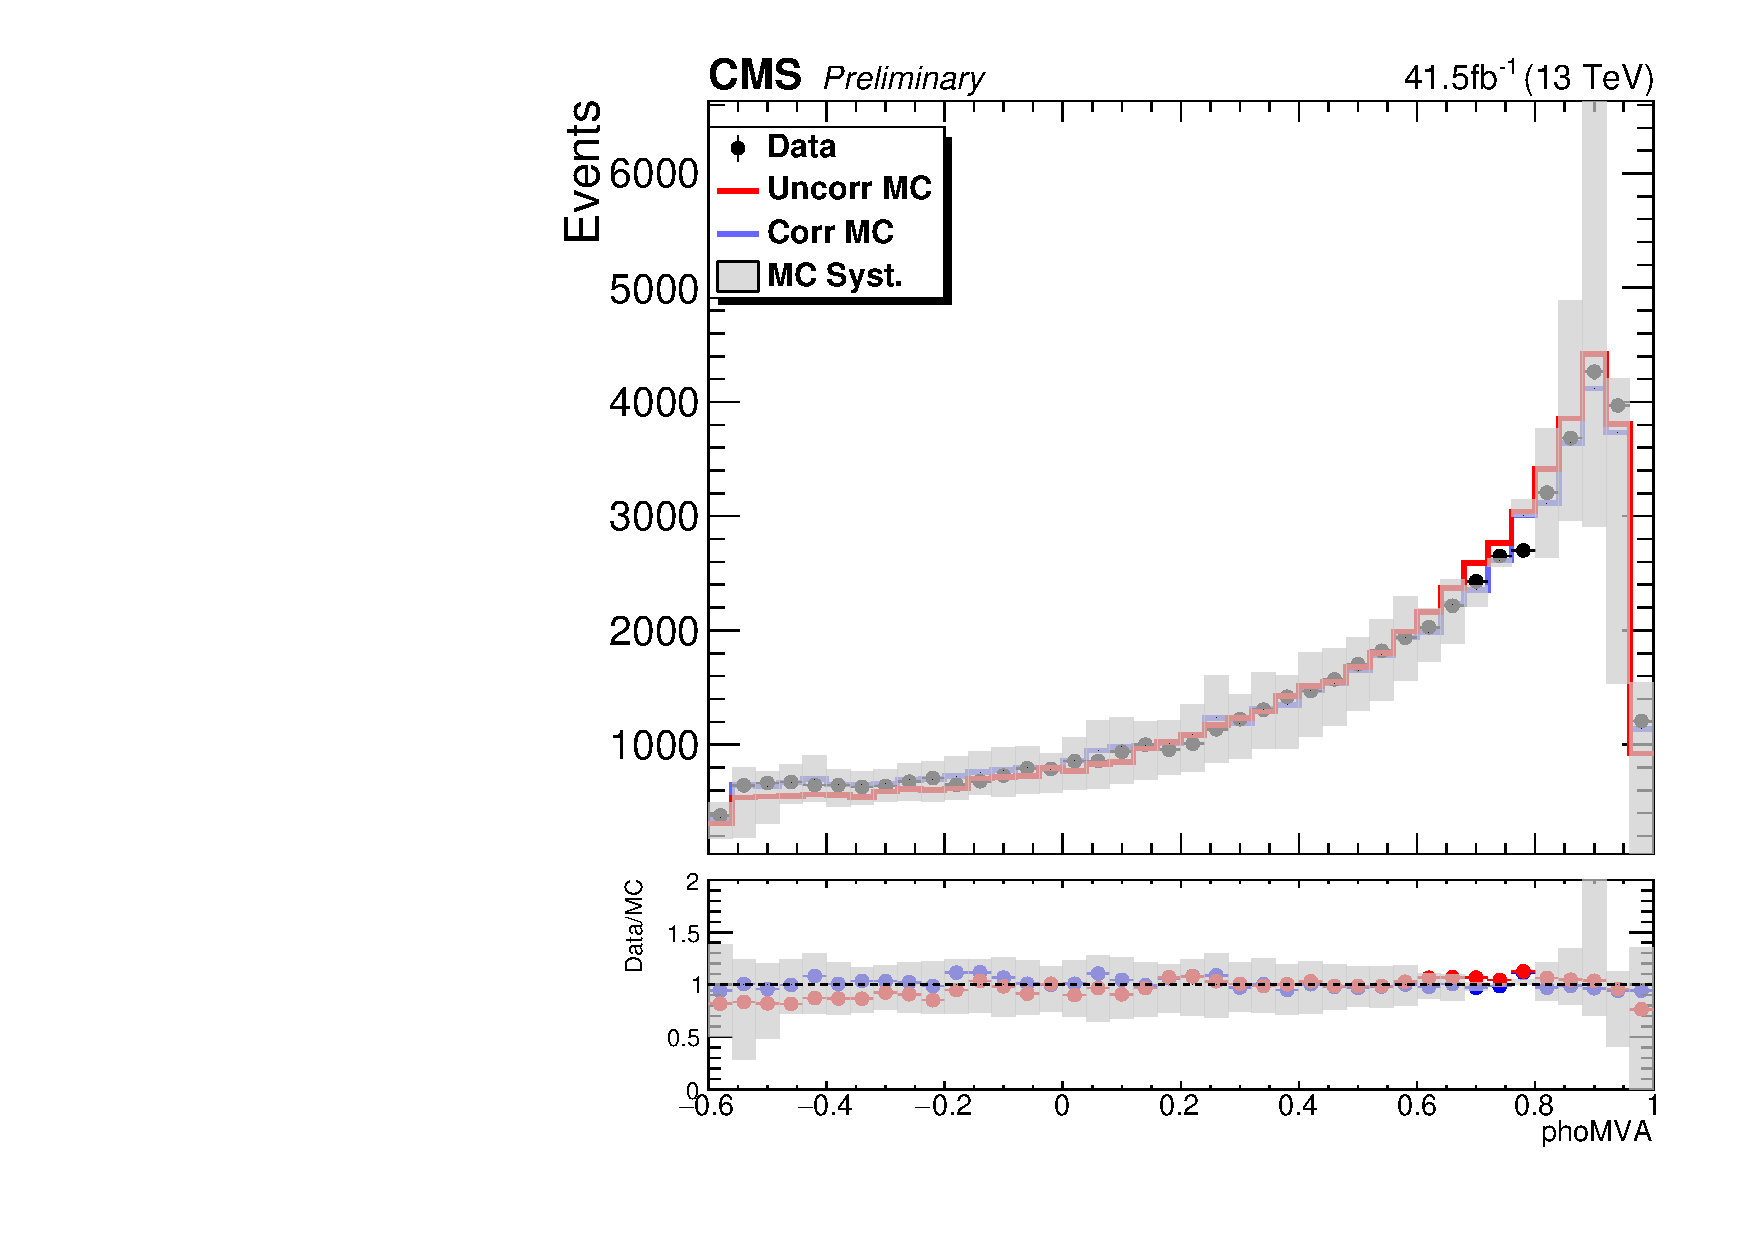
\includegraphics[width=0.35\textwidth]{fig/ss_corr/phoMVA_17_EE_Z_mmg.pdf}
	\end{center}
	\caption{Comparison of simulation with 2017 data for the photon MVA ID before and after shower shape corrections are applied to the simulation. The plots on the left (right) correspond to the barrel and endcap regions, and the upper (lower) plots correspond to $\PZ\to\epem$ ($\PZ\to\mpmm+\PGg$) events.}
	\label{fig:photon_mva_correction}
\end{figure}

Based on the corrected photon MVA ID, 90\% signal efficiency working point (WP) cuts for barrel and endcap photons 
are determined for the \hzg{} analysis. The WPs are defined based on real photons from $\Z\gamma$ simulation, and correspond 
to photon MVA ID scores greater than -0.4 (-0.59) for barrel (endcap) photons. 
These relatively loose cuts are chosen because the photon MVA ID is later used as an input to a BDT for categorization, as described in 
the next chapter.
A comparison of these WPs with the general CMS 90\% efficiency WPs, 
plotted on the receiver operator characteristic (ROC) curve for $\PZ\gamma$ (signal) and $\PZ$+jets (background)
simulation, is shown in Fig. \ref{fig:photon_mva_roc}. The efficiency of the photon MVA ID is measured with $\PZ\to\epem$ data
using a tag and probe technique. The tag electron must pass the single electron trigger with \pt threshold 27 (32) GeV in 
2016 (2017 and 2018), pass a tight cut-based identification, have \pt $>$ 30 (35) GeV for 2016 (2017 and 2018), and have $|\eta| < 2.5$. The 
probe electron must pass the corrected photon MVA ID. The corresponding SFs, measured and 
applied in bins of \pt and supercluster $\eta$, are shown in Fig. \ref{fig:photon_id_sf}. The efficiencies and SFs for the conversion-safe 
electron veto are measured by CMS using $\PZ\to\mpmm$ events with an FSR photon and are applied in the \hzg{} analysis. 
These SFs are cataloged in Table \ref{tab:eveto_sf}. 

\begin{figure}[tb]
	\begin{center}
		\includegraphics[width=0.75\textwidth]{fig/selection/photon_ID_ROC.png}
	\end{center}
	\caption{ROC curves for the corrected photon MVA ID in the barrel (red) and endcaps (blue). Here, signal refers to real photons from the $\PZ\PGg$ simulation and background refers to jets misreconstructed as photons from the $\PZ$+jets simulation. Also shown are the cuts used for the \hzg{} analysis WP and for the standard CMS 90\% WP.}
	\label{fig:photon_mva_roc}
\end{figure}

\begin{table}[tb]
	\centering   
\caption{Photon conversion-safe electron veto SFs.}
	\begin{tabular}{|c|cccccc|}

	\hline
	&\multicolumn{3}{c}{barrel} &\multicolumn{3}{c|}{endcap}\\
&0--30\GeV &30--60\GeV&60--200\GeV&0--30\GeV &30--60\GeV&60--200\GeV\\\hline
2016&\multicolumn{3}{c}{0.9938}&\multicolumn{3}{c|}{0.9875}\\
2017&\multicolumn{3}{c}{0.967}&\multicolumn{3}{c|}{0.915}\\
2018&0.987613&0.98895& 1.00006&0.95461&0.962451&0.99791\\\hline
	\end{tabular}
\label{tab:eveto_sf}
\end{table}

\begin{figure}[tb]
	\begin{center}
		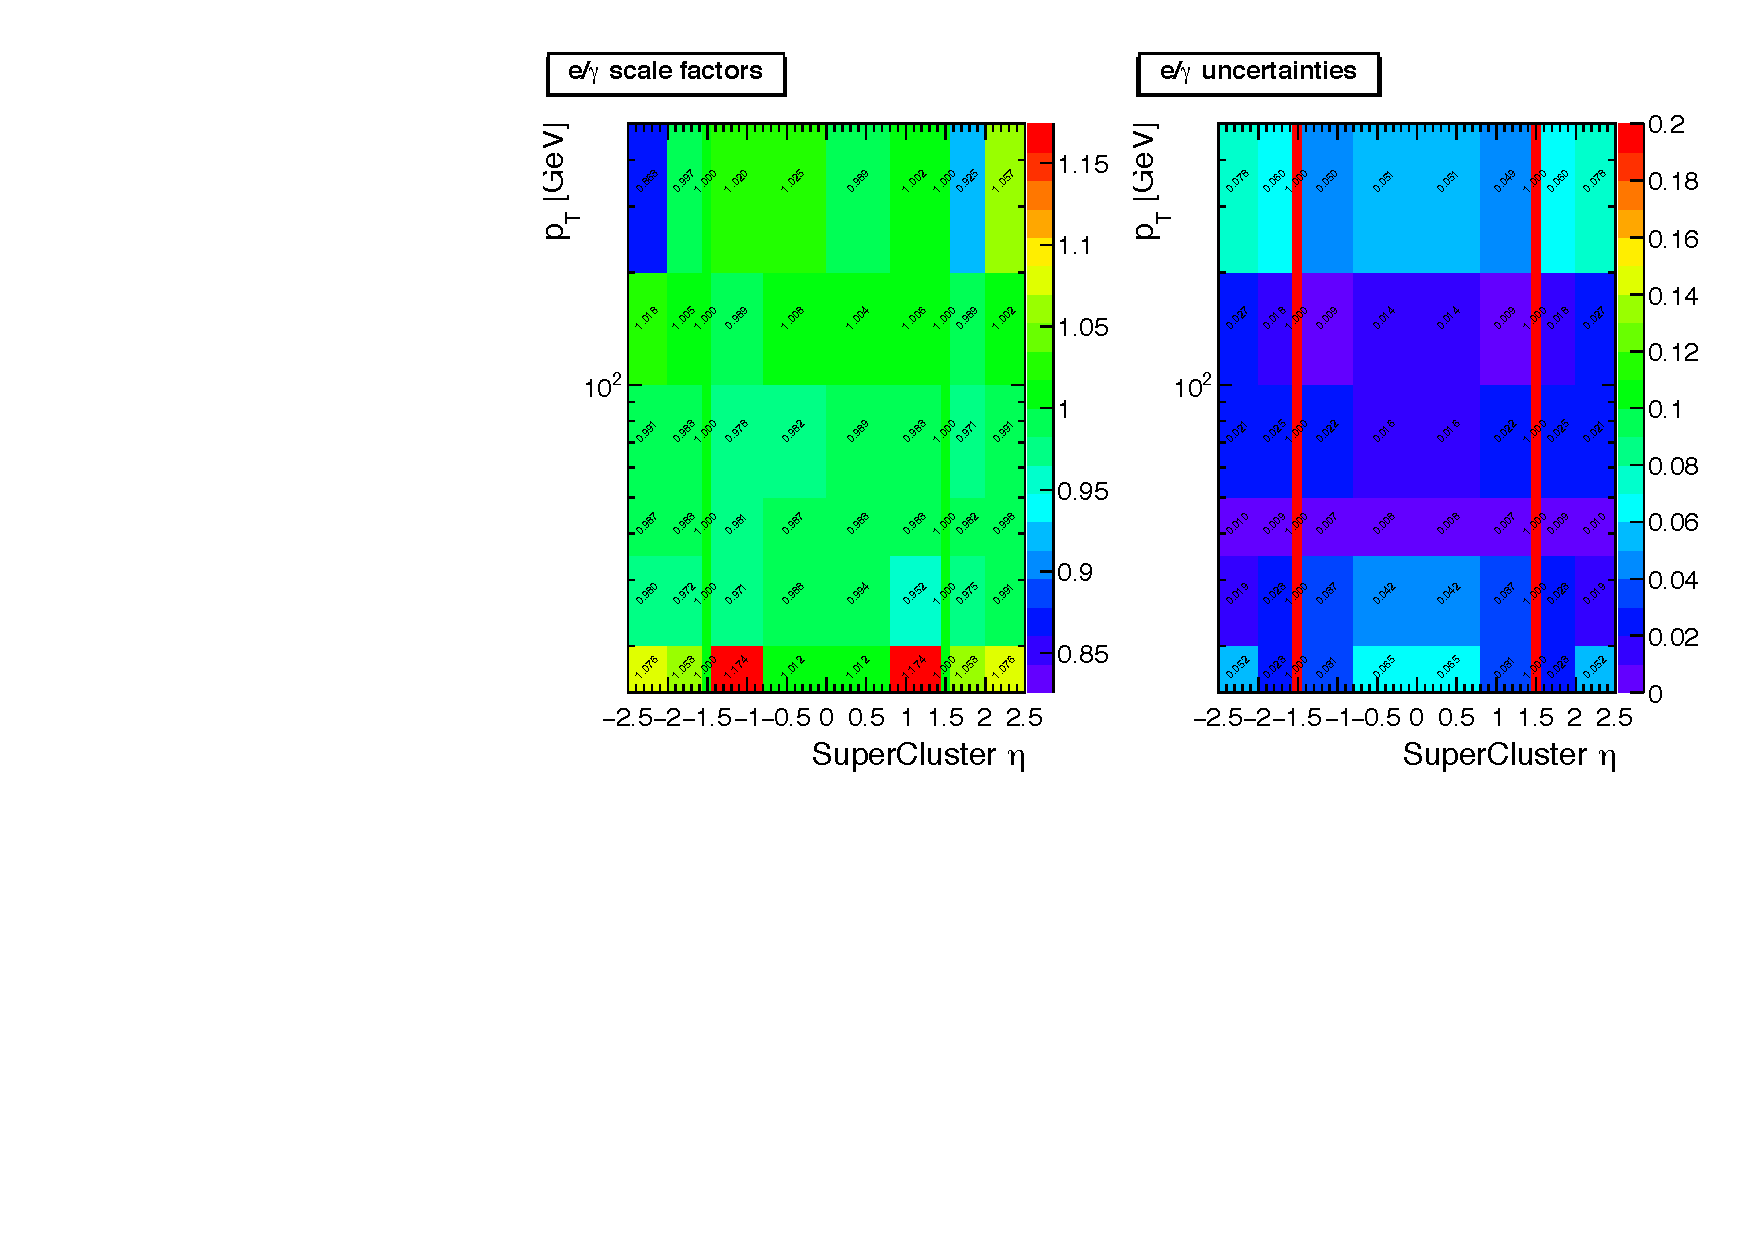
\includegraphics[width=0.6\textwidth]{fig/SFs/2016_ID_pho_2D.pdf}
		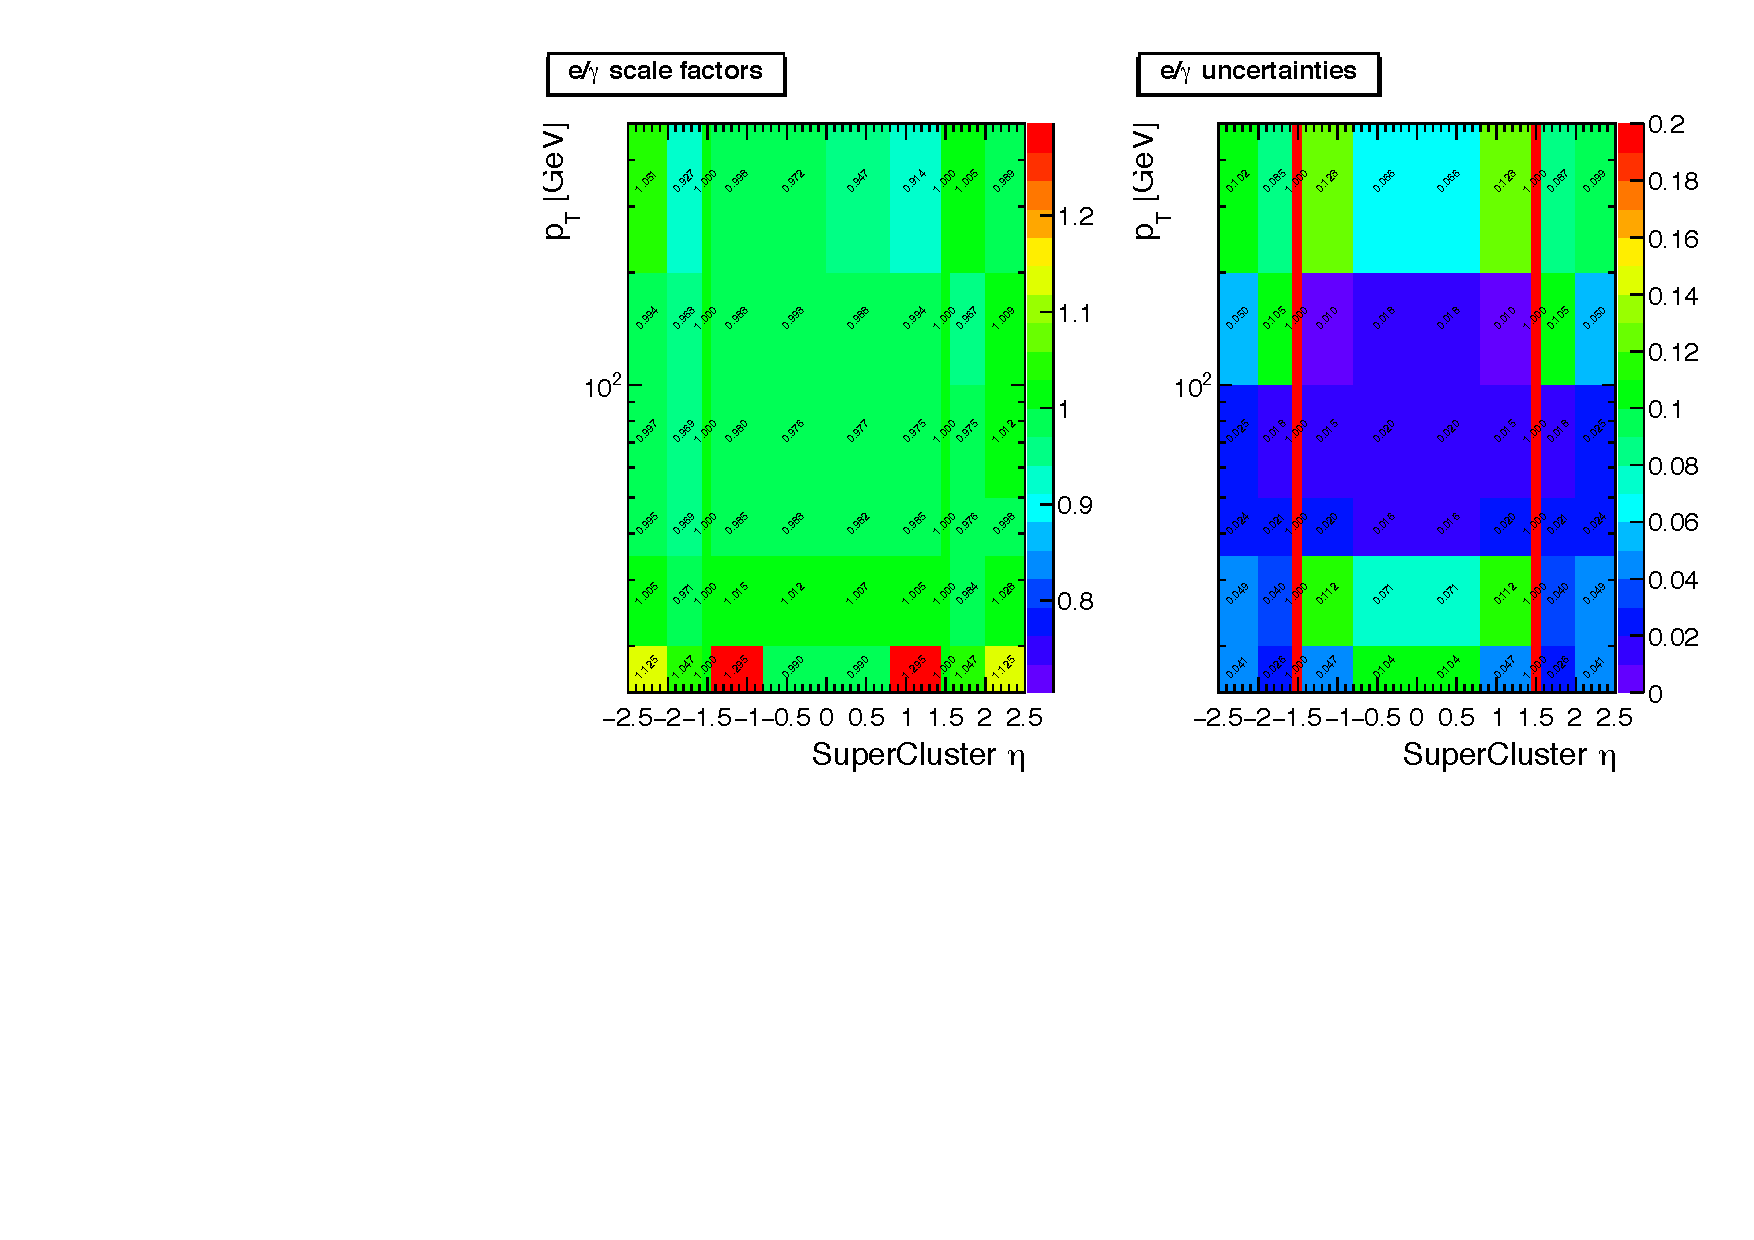
\includegraphics[width=0.6\textwidth]{fig/SFs/2017_ID_pho_2D.pdf}
		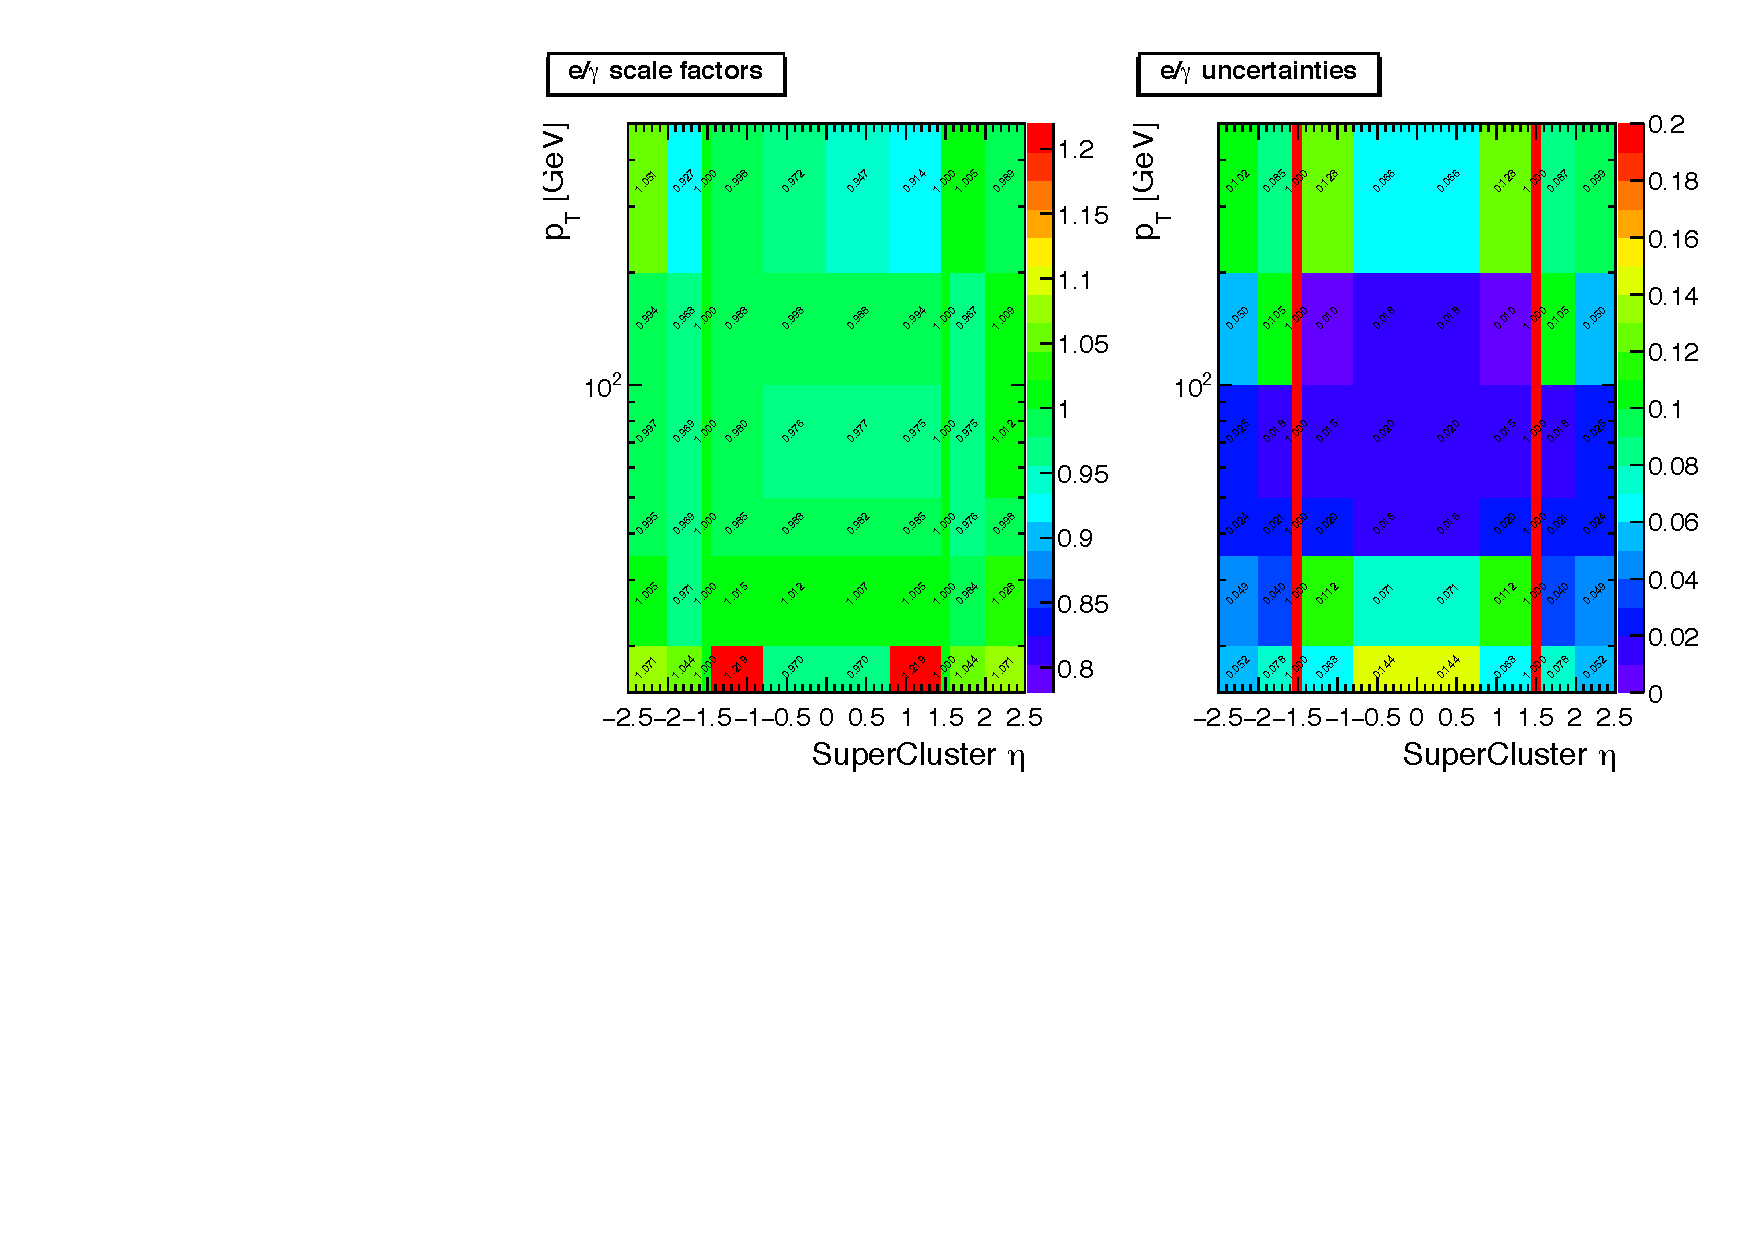
\includegraphics[width=0.6\textwidth]{fig/SFs/2018_ID_pho_2D.pdf}
	\end{center}
	\caption{Left: Photon MVA ID efficiency SFs for 2016 (upper), 2017 (middle), and 2018 (lower). Right: The corresponding uncertainties for the SFs.}
	\label{fig:photon_id_sf}
\end{figure}


\clearpage

\section{Electron Selection}
Electrons are identified using a BDT discriminant (electron MVA ID) trained on Drell--Yan plus jets simulation, 
with prompt electrons matched to generator-level objects as signal and unmatched and non-prompt electrons as background. The features 
used in the BDT training include \pt, supercluster $\eta$, shower shape variables, ratio of hadronic to electromagnetic energy, track and 
pixel hit variables, and isolation variables~\cite{EGM:ElectronID}. 
Since isolation features are included in the training of the photon MVA ID, there is no need for a separate isolation requirement. 
For the \hzg{} analysis, an electron is selected if its photon MVA ID score is higher than a loose WP
value, corresponding to 98\% signal efficiency. In addition to the photon MVA ID cut, electrons must satisfy the impact parameter requirements $|d_{xy}| < 0.5$ cm and $|d_{z}| < 1$ cm
with respect to the PV. 

Electron MVA ID efficiencies and SFs are measured using a tag and probe method on dielectron events near the 
$\PZ$ boson mass peak. The electrons used by this procedure are required to pass the single electron trigger with a \pt threshold of 27 (32) GeV for 2016 (2017 and 2018) data. 
The dielectron mass must be in the range 60--120\GeV. The tag electron must pass a tight cut-based electron ID and have 
$\pt>30\,(35)\GeV$ for 2016 (2017 and 2018) and $|\eta|<2.5$. The probe electron is required to pass the loose electron MVA ID cut and the
impact parameter cuts described above. Identification efficiencies and SFs are measured and applied in bins of 
\pt and supercluster $\eta$. The SFs for each data-taking year are shown in Fig. \ref{fig:electron_id_sf}.

\begin{figure}[tb]
	\begin{center}
		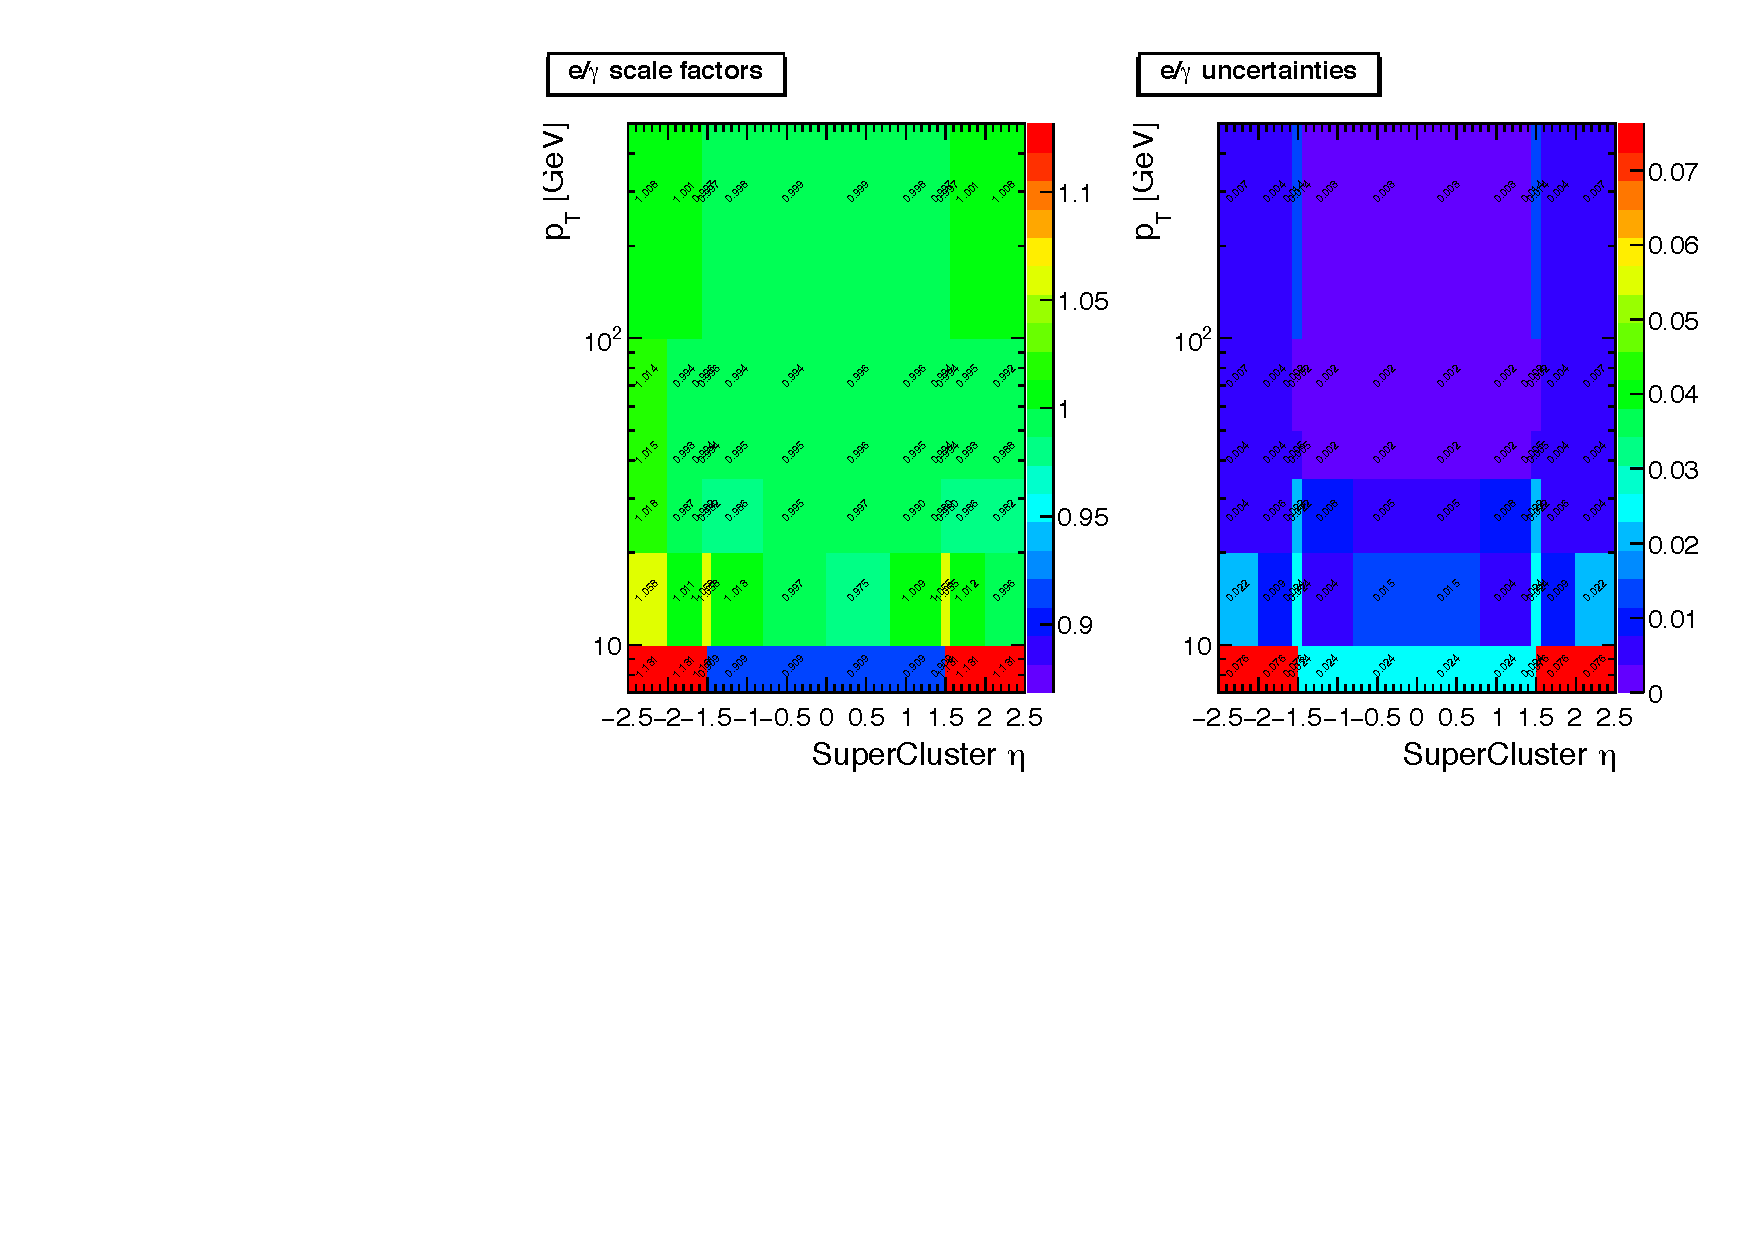
\includegraphics[width=0.6\textwidth]{fig/SFs/2016_ID_ele_2D.pdf}
		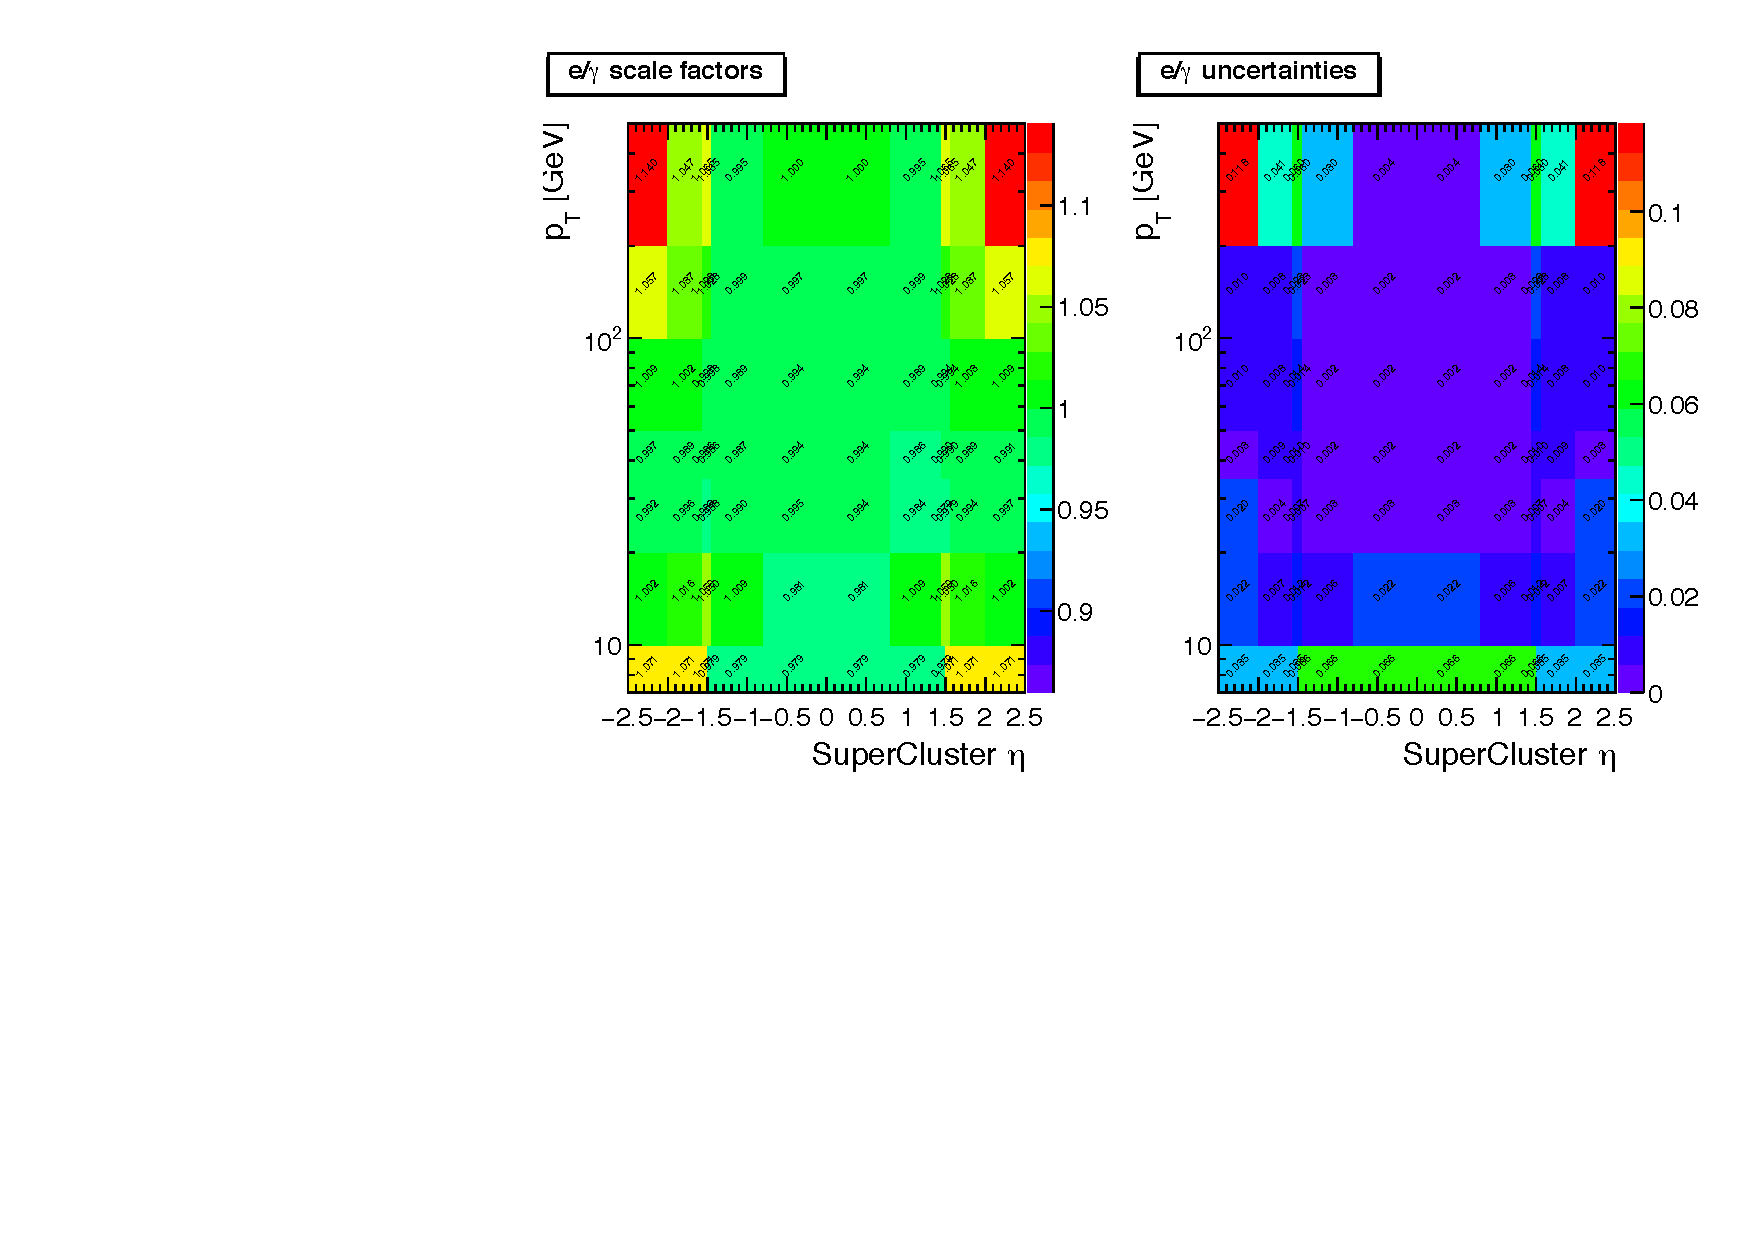
\includegraphics[width=0.6\textwidth]{fig/SFs/2017_ID_ele_2D.pdf}
		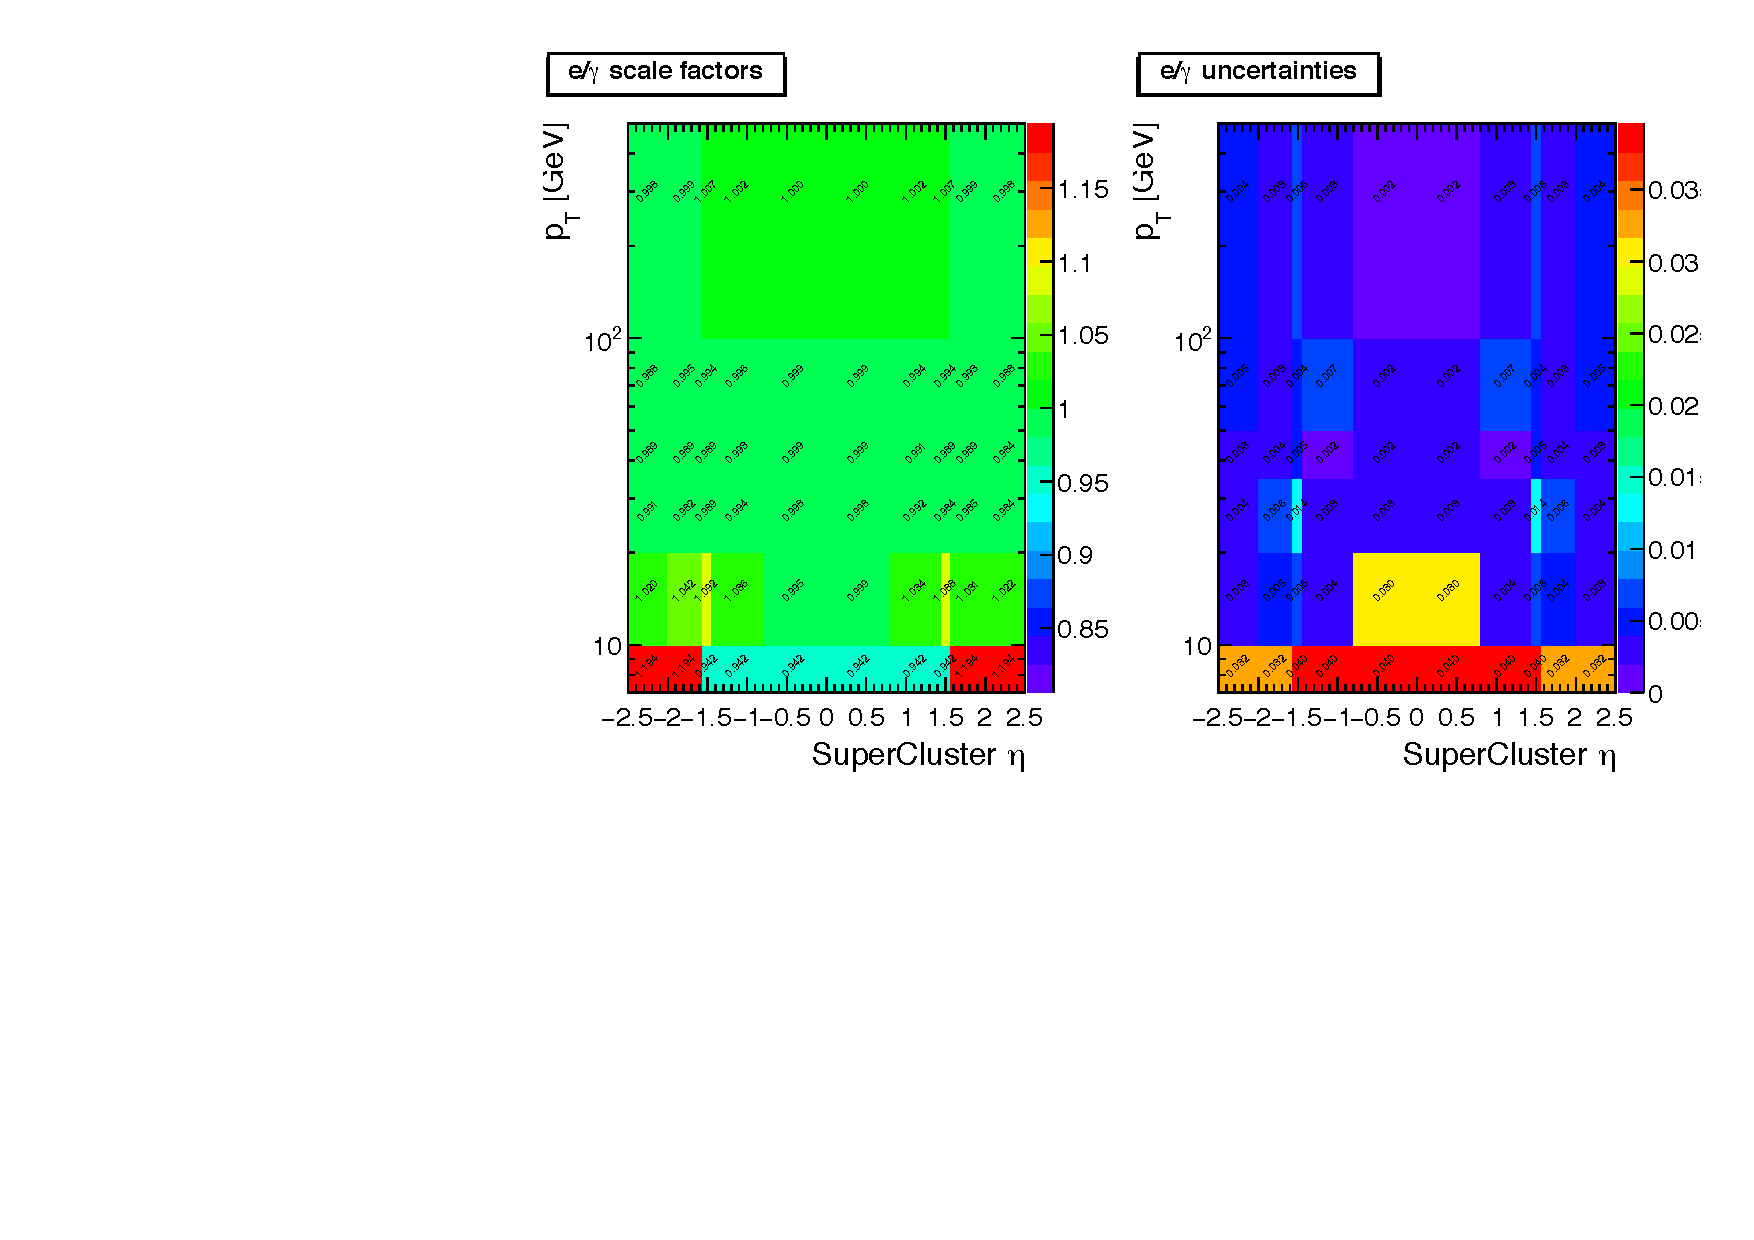
\includegraphics[width=0.6\textwidth]{fig/SFs/2018_ID_ele_2D.pdf}
	\end{center}
	\caption{Left: Electron MVA ID efficiency SFs for 2016 (upper), 2017 (middle), and 2018 (lower). Right: The corresponding uncertainties for the SFs.}
	\label{fig:electron_id_sf}
\end{figure}

\clearpage

\section{Muon Selection}
A loose cut-based muon identification is used in this analysis. This ID was originally developed for the CMS $\PH\to\PZ\PZ^*\to4\ell$ analysis of the 2016 data set~\cite{bib:htozz2016} and is well-suited for \hzg{} due to the similar kinematics of the multiple muons in the final state. 
All muons are first required to pass a set of common ID cuts, followed by a separate set of cuts for high ($>200\GeV$)
and low \pt muons. All muons are required to satisfy $|\eta| < 2.4$, $|d_{xy}| < 0.5$ \cm, and $|d_{z}| < 1$ \cm, where
the impact parameters are defined with respect to the PV using the best fit muon track. 
Additionally, the three-dimensional impact parameter with respect to the PV must have a magnitude less than four times its uncertainty.
Muons are required to either be reconstructed as global muons or tracker muons. Those with standalone tracks only in the muon system are
rejected. 
Low \pt muons satisfying the common requirements of the PF ID algorithm are selected. 
High \pt muons are selected if they pass the PF ID or if they pass
the following high \pt requirements: the muon is matched to segments in at least two muon 
stations; satisfies $\frac{p_{T}}{\sigma_{p_{T}}} < 0.3$, $|d_{xy}| < 0.2$ cm, $|d_{z}| < 0.5$ cm; has at least one pixel hit; and has
tracker hits in at least six tracker layers.

A relative PF isolation requirement is imposed, defined by the variable
\begin{equation}
\label{eqn:pfiso}
	\mathcal{I}^{\mu} \equiv \Big[ \sum \pt^\text{charged} +
                                 \max\big( 0, \sum \pt^\text{neutral}
                                 +
                                  \sum \pt^{\Pgg}
                                 - \pt^{\mu\mathrm{,PU}} \big) \Big]
                                 / \pt^{\mu}.
\end{equation}
The quantity $\sum \pt^\text{charged}$ is the scalar sum of the \pt
of charged hadrons originating from the PV,
and $\sum \pt^\text{neutral}$ and $\sum \pt^{\Pgg}$ are the scalar sums of the \pt of neutral hadrons and photons, respectively. 
The sums are over all PF candidates within a cone of radius $\DR = 0.3$ around the photon or lepton direction at the PV. 
Muons are required to satisfy $\mathcal{I}^{\mu} < 0.35$. 
The ID and isolation efficiencies and SFs with uncertainties were measured and provided by the CMS $\PH\to\PZ\PZ^*\to4\ell$ analysis working group.

In 2016, data-taking was affected by a problem in which the L1 trigger sent only one candidate per 60$^{\circ}$ sector instead 
of up to three~\cite{twiki:l1emtf}. As a result, when two muons in the same endcap had a low $\Delta \phi$ separation, only one would fire the 
trigger. To account for this, 2016 data events containing identified muons with $\Delta \phi < 70^{\circ}$ in the same endcap region 
are rejected. 


\section{Jet Selection}
Jets are selected in order to categorize events coming from potential VBF Higgs production, but there is no jet muliplicity requirement 
for the \hzg{} event selection. In fact, the majority of simulation and data events selected in the analysis have no jets. However, identifying 
and selecting jets to categorize VBF events can still significantly improve the sensitivity of the search. Jets are required to pass 
a loose cut-based identification in 2016 and a tight cut-based identification in 2017 and 2018. 
Additionally, jets must satisfy $\pt>30\GeV$, $|\eta| < 4.7$, and $\Delta R > 0.4$ with 
respect to each lepton and the photon selected in the analysis. An issue with noise in the ECAL endcaps in 2017~\cite{eenoise} caused an artificial 
increase in jet multiplicity in data within a specific kinematic phase space. To mitigate this, jets are rejected if they have 
uncorrected \pt $<$ 50 GeV and $2.65 < |\eta| < 3.139$. This cut reduces the efficiency to reconstruct dijet pairs by 12\% in the specified 
region. To tag VBF events, we are interested in dijet pairs. If there are more than two jets satisfying the above criteria, 
only the two highest \pt jets are selected. No SFs are needed for these jet selection requirements as they do not impact the event selection.

\section{Object Corrections}
Several corrections are applied to the physics objects selected in the analysis. Rochester muon momentum scale and resolution 
corrections~\cite{muonRoc} are applied to both data and simulation. This greatly improves the calibration of the dimuon mass near the $\PZ$ boson peak, as shown in Fig. \ref{fig:rochester}. 
Energy scale and resolution corrections for electrons, photons, and jets are also applied in the analysis. The procedures for these corrections and the corresponding SFs for simulation 
are provided by CMS.

\begin{figure}[tb]
	\begin{center}
		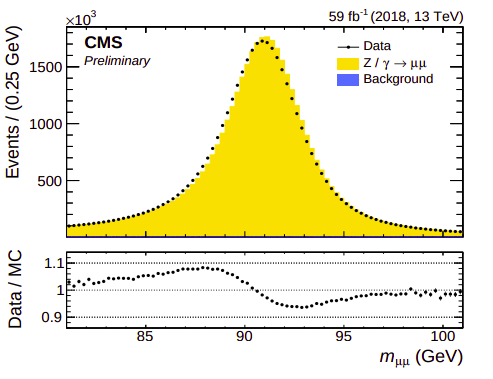
\includegraphics[width=0.45\textwidth]{fig/selection/roccor_before.png}
		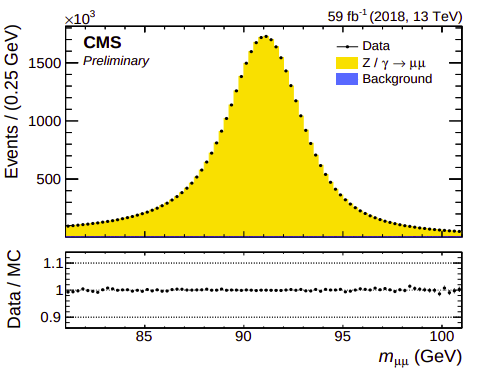
\includegraphics[width=0.45\textwidth]{fig/selection/roccor_after.png}
	\end{center}
	\caption[Dimuon invariant mass around the $\PZ$ boson peak in 2018 data before (left) and after (right) the muon Rochester momentum corrections are applied.]
	{Dimuon invariant mass around the $\PZ$ boson peak in 2018 data before (left) and after (right) the muon Rochester momentum corrections are applied~\cite{muonRoc}.}
	\label{fig:rochester}
\end{figure}

An FSR recovery procedure is performed for the selected muons, 
following a similar approach to that used in Ref.~\cite{bib:htozz2016}. An FSR photon is 
identified and associated to its radiating muon based on the following criteria. The 
photon must satisfy $\pt>2$\GeV, $\lvert{\eta}\rvert < 2.4$, $\DR(\gamma,\mu)/p_{\mathrm{T}\gamma}^{2} < 0.012 \GeV^{-2}$, $\DR(\gamma,\mu) < 0.4$, and relative PF isolation smaller than 1.8, where the pileup contribution is excluded from the isolation calculation. If 
multiple FSR photons are associated to one muon, the photon with the smallest 
value of $\DR(\gamma,\mu)/p_{\mathrm{T}\gamma}^{2}$ is selected. 
In simulation, we find that the selected FSR photon matches the generator level FSR photon with 93\% efficiency. 
Figure \ref{fig:fsr_recovery} shows the dilepton and $\lplm\PGg$
invariant mass among FSR photon-containing signal events with and without applying the FSR recovery correction.
The FSR recovery procedure improves the $m_{\lplm\gamma}$ resolution by 1\% in the muon channel.

\begin{figure}[tb]
	\begin{center}
		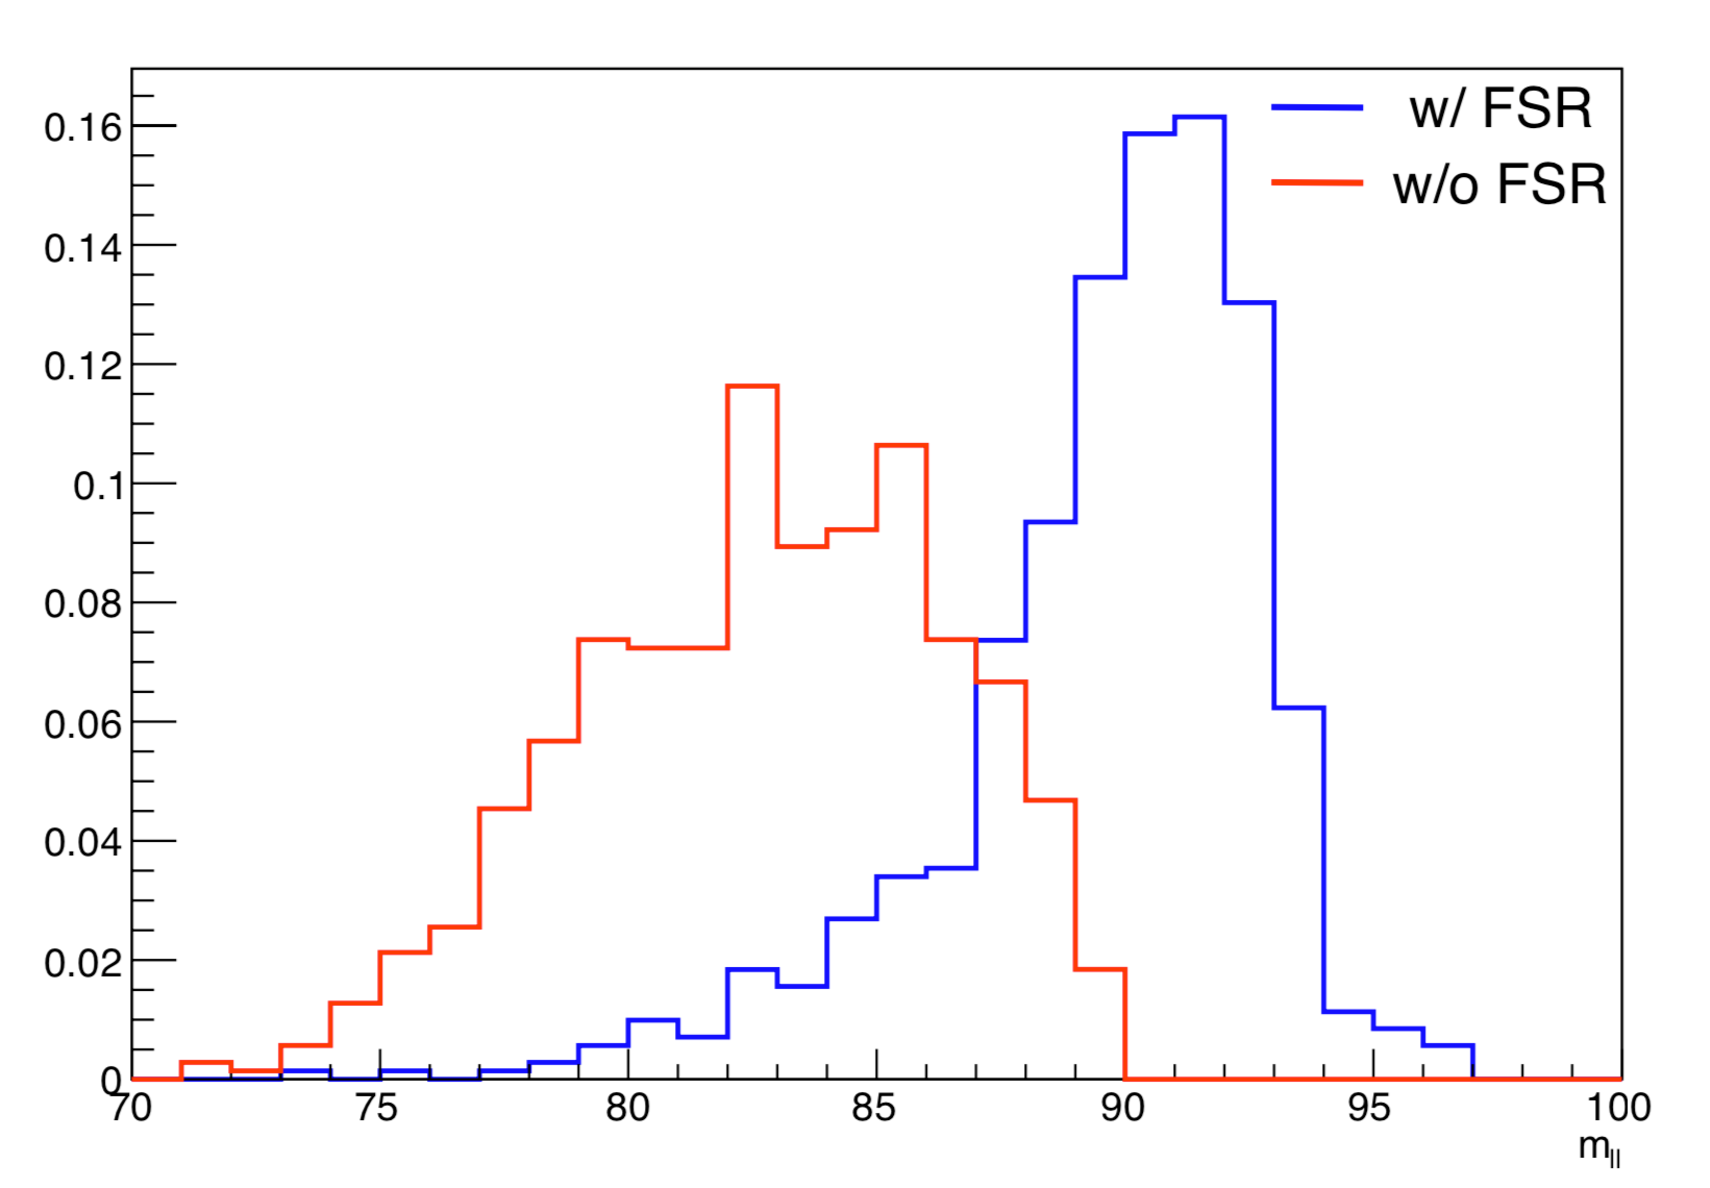
\includegraphics[width=0.45\textwidth]{fig/selection/mll.pdf}
		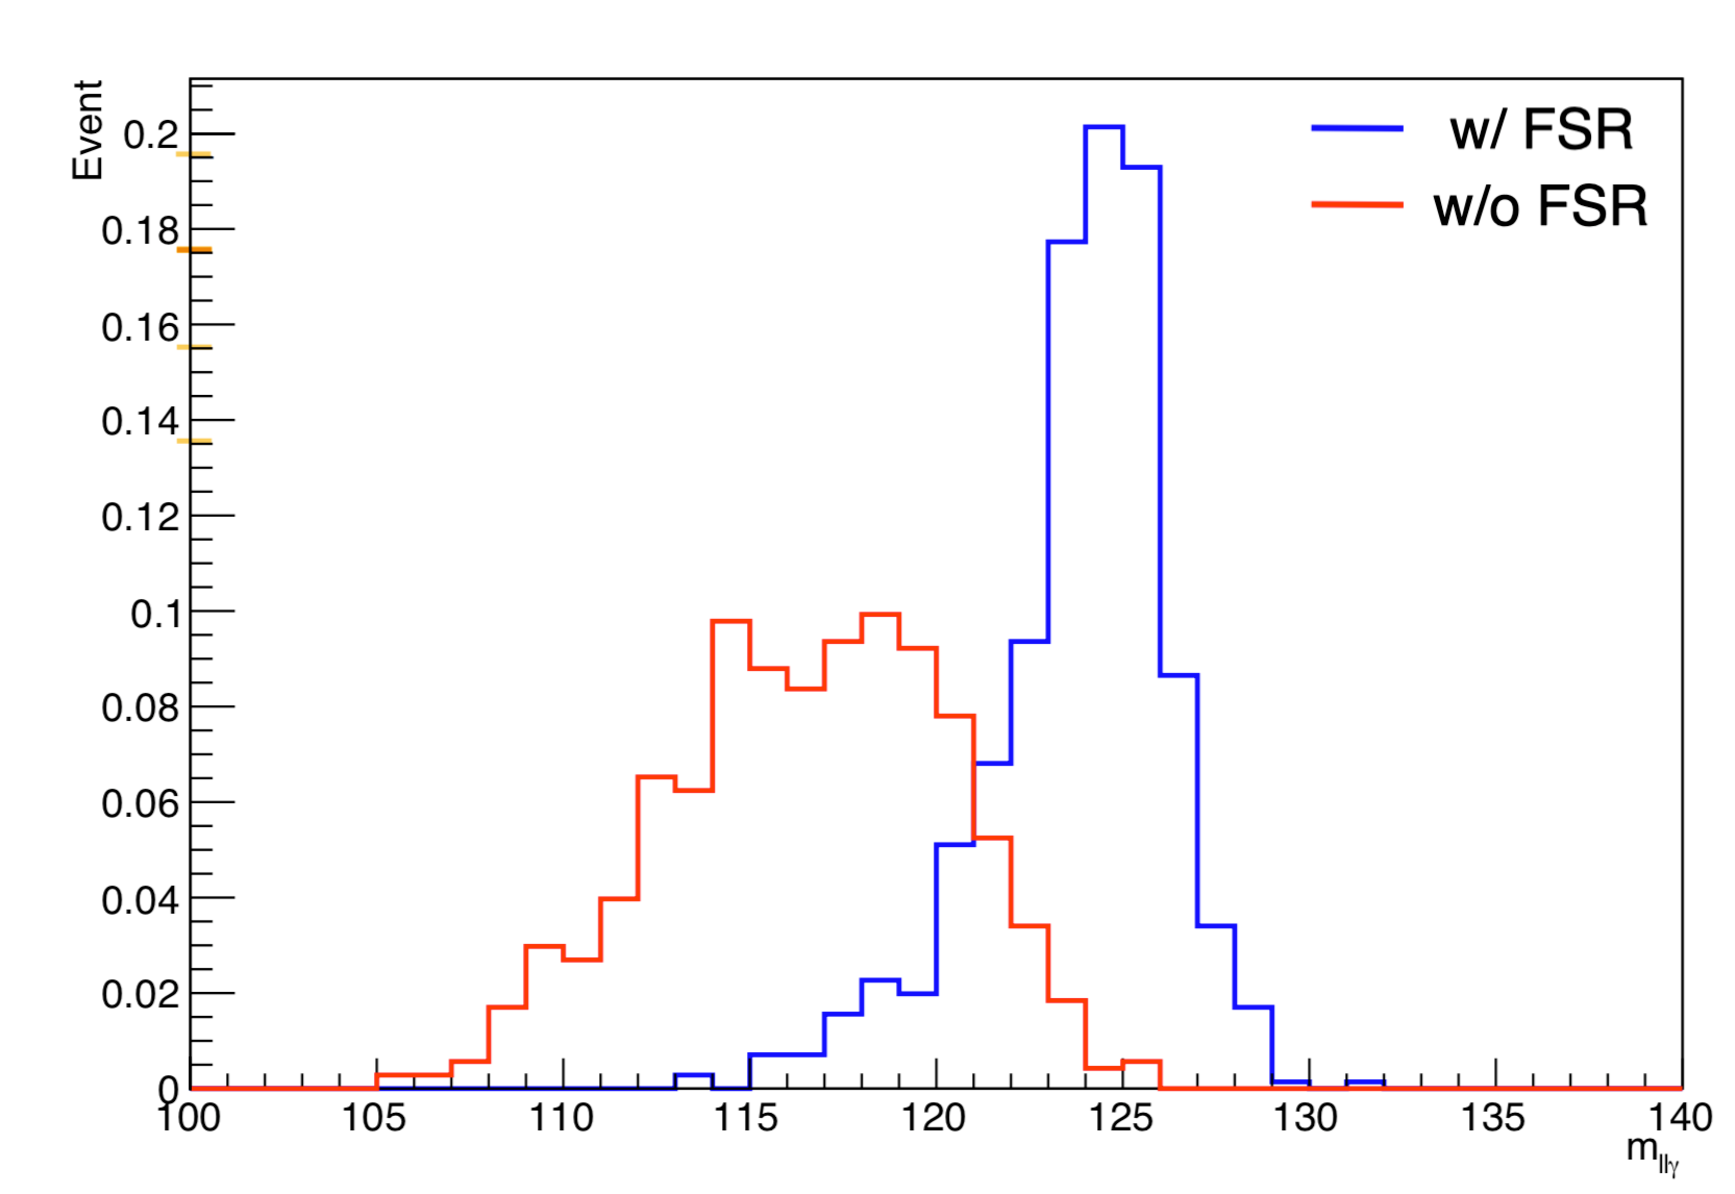
\includegraphics[width=0.45\textwidth]{fig/selection/Hmass.pdf}
	\end{center}
	\caption{Dilepton invariant mass (left) and $\lplm\gamma$ invariant mass (right) with (blue) and without (red) FSR photon recovery for simulated $\PH\to\PZ\gamma\to\mpmm\gamma$ events containing at least one FSR photon.}
	\label{fig:fsr_recovery}
\end{figure}

\section{Event Selection}
Events are required to contain a photon and at least two same-flavor, oppositely charged leptons ($\ell = \Pe$ or $\mu$) with $m_{\lplm}>50$\GeV.  
The dilepton mass requirement, although relatively loose, is sufficient to suppress backgrounds that do not contain $\PZ$ boson decays while retaining high signal efficiency. The particles used to reconstruct the $\PZ\gamma$ candidate system are required to have $\pt > 25\,(15)$\GeV for the leading (subleading) electron, $\pt > 20\,(10)$\GeV for the leading (subleading) muon, and $\pt > 15$\GeV for the photon. 
The photon must also satisfy $0 < |\eta| < 1.4442$ or $1.566 < |\eta| < 2.5$. 
This avoids the calorimeter transition region, in which photon reconstruction is more difficult. 
In events with multiple dilepton pairs, the pair with 
mass closest to the nominal $\PZ$ boson mass~\cite{PhysRevD.98.030001} is selected. Additional electrons (muons) with \pt greater than 7 (5)\GeV are also used for categorization, as described in the next chapter. 

The invariant mass of the $\lplm\gamma$ system is required to be in the range $105 < m_{\lplm\gamma} < 170$\GeV, which provides a broad range around the Higgs boson mass in which to perform the fit.
%  to be consistent with the Higgs boson mass.
Events are required to have a photon satisfying $\pt^\gamma / m_{\lplm\gamma} > 0.14$,
which suppresses the $\PZ$+jets background 
without significantly reducing signal efficiency, with minimal bias in the
$m_{\lplm\gamma}$ spectrum. Each lepton is required to have $\DR>0.4$
with respect to the photon to reject events with FSR. To further reject FSR from $\PZ\gamma$
processes, we require $m_{\lplm\gamma} + m_{\lplm} > 185\GeV$. 

\section{Kinematic Fit}
A kinematic fit procedure is used to improve the dilepton mass and $m_{\lplm\gamma}$ resolutions, 
following a similar 
approach to that used in Ref.~\cite{bib:htozz2016}. A maximum likelihood fit is performed, taking into account 
the true $\PZ$ boson line shape, obtained from \hzg{} simulation, the \pt of each lepton, 
and the \pt resolution of each lepton. The outputs of this fit are the corrected \pt values for each 
lepton. The likelihood function for the fit is given by

\begin{equation}
	\mathcal{L}(\ptone,\pttwo|\ptoner,\sigma_{\ptone},\pttwor,\sigma_{\pttwo}) = \mathcal{N}(\ptoner|\ptone,\sigma_{\ptone})\cdot\mathcal{N}(\pttwor|\pttwo,\sigma_{\pttwo})\cdot\mathcal{L}(m_{12}|m_{\PZ}),
\end{equation}
where $\mathcal{N}$ represents the normal distribution, \ptoner and \pttwor are the reconstructed transverse momenta of the two leptons, 
$\sigma_{\ptone}$ and $\sigma_{\pttwo}$ are the per-lepton transverse momentum resolutions, 
$\ptone$ and $\pttwo$ are the corrected \pt values, $m_{12}$ is the invariant mass 
calculated from $\ptone$ and $\pttwo$, and $\mathcal{L}(m_{12}|m_{\PZ})$ is the likelihood given the true Z mass lineshape. 
The corrected \pt values are used to recalculate the dilepton mass and $m_{\lplm\gamma}$. 
Figure \ref{fig:kinfit} shows the dilepton mass distributions before and after the kinematic fit.
The improvement in signal $m_{\lplm\gamma}$ resolution varies with data-taking year and is between 
20--27\% in the electron channel and 10--12\% in the muon channel. The effect of the 
kinematic fit is larger for the electron channel because of the poorer momentum resolution for electrons compared to muons. 

\begin{figure}[tb]
	\begin{center}
		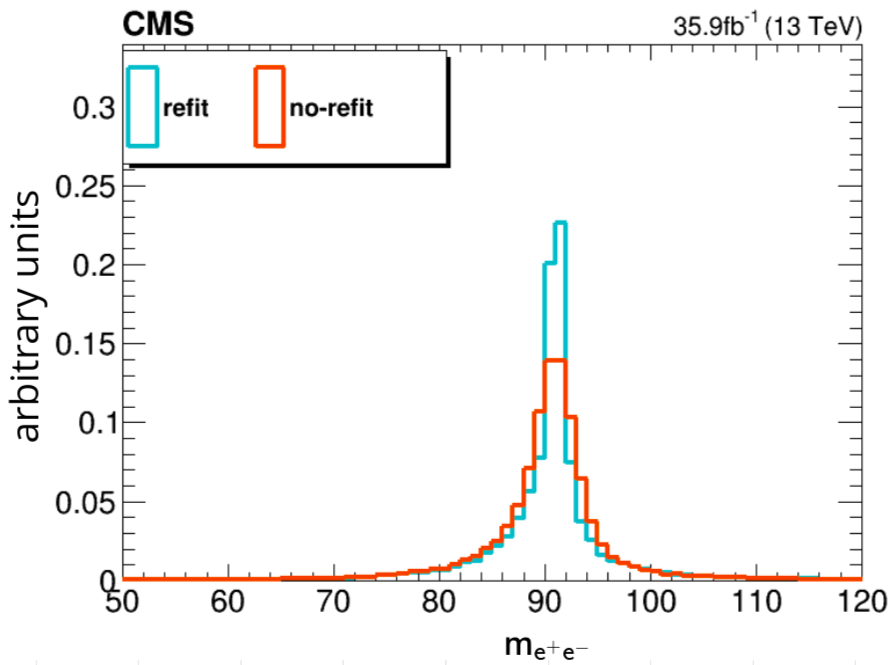
\includegraphics[width=0.45\textwidth]{fig/selection/kinfit_data_el.png}
		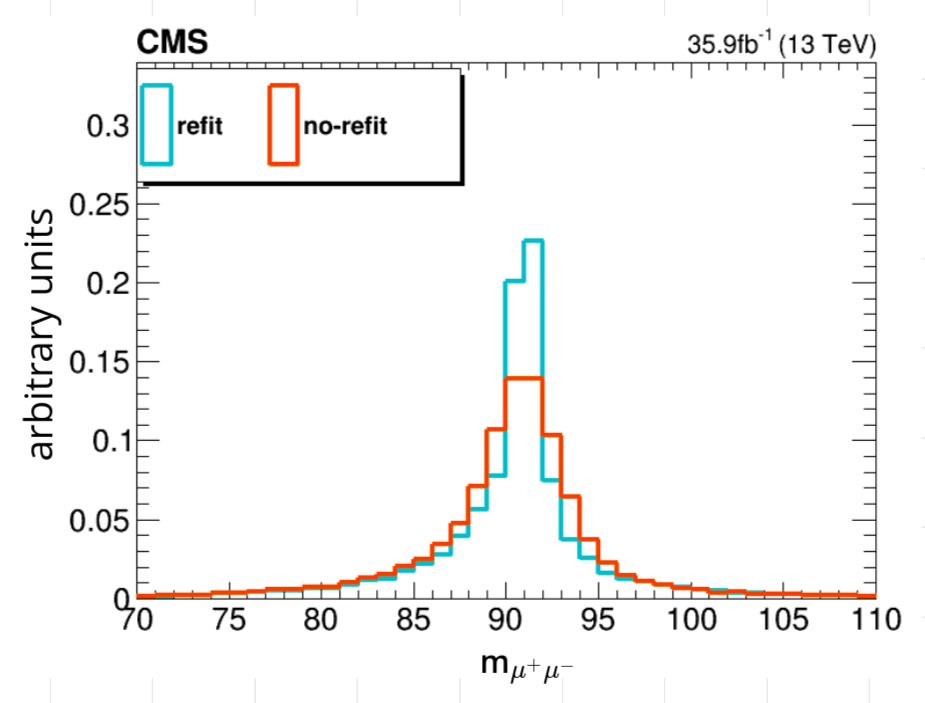
\includegraphics[width=0.45\textwidth]{fig/selection/kinfit_data_mu.png}
	\end{center}
	\caption{Dilepton invariant mass in 2016 data before and after the kinematic fit for the electron (left) and muon (right) channels.}
	\label{fig:kinfit}
\end{figure}

\section{Yields and Kinematic Distributions}
